\documentclass[journal]{IEEEtran}

\usepackage{amsmath,amssymb,amsfonts}
\usepackage{graphicx}
\usepackage{booktabs}
\usepackage{cite}
\usepackage{algorithm}
\usepackage{algorithmic}

\newcommand{\E}{\mathbb{E}}
\newcommand{\Prb}{\Pr}
\newcommand{\median}{\mathrm{median}}
\newcommand{\R}{\mathbb{R}}
\newcommand{\Cset}{\mathcal{C}}
\newcommand{\N}{\mathcal{N}}

\author{\IEEEauthorblockN{Zhiguo Xiao\textsuperscript{1,2,*},
Yujing Guo\textsuperscript{2}, Yanqi Shao\textsuperscript{2},
Guangteng Chen\textsuperscript{2}, Dingbo Hou\textsuperscript{2},
Yuanyuan Liu\textsuperscript{2}, Xinyao Cao\textsuperscript{2}, Junli Liu\textsuperscript{2}}
\IEEEauthorblockA{\textsuperscript{1}School of Computer Science and Technology,
Beijing Institute of Technology, Beijing 100811, China\\
\textsuperscript{2}School of Computer Science and Technology,
Changchun University, Changchun 130022, China}
\IEEEauthorblockA{\textsuperscript{*}Corresponding author: Zhiguo Xiao
(email: 3220215169@bit.edu.cn)}}

\title{Separating Failure-Bound Degradation from Benign Drift:\\A Rate-Normalized Early-Warning Detector\\with Fleet-Scale False-Alarm Analysis}

\markboth{IEEE Internet of Things Journal}%
{Xiao \MakeLowercase{\textit{et al.}}: Rate-Normalized Early-Warning Detector}

\begin{document}
\maketitle

\begin{abstract}
Early failure warning for rotating machinery in industrial IoT must separate failure-bound degradation from benign drift, under a zero-false-alarm constraint, at millisecond scale on edge nodes. We reduce the discriminative signal to the cumulative excess of root-mean-square amplitude above a $1.2\times$ early-life baseline, interpreted as a deployable coarse-grained observable of monotone damage accumulation. It fully separates the four failed from the eight censored NASA IMS bearings (exact permutation $p=1/495$, the minimum attainable), read as mechanistic evidence, not a performance claim. Its causal online form, the rate-normalized time-averaged excess with one fixed threshold, detects 31 of 34 failed bearings (95\% CI 76.3--98.1\%) across IMS, XJTU-SY, and FEMTO/PRONOSTIA, with median lead times of 14.5\%, 46.3\%, and 36.0\% of life, calibrated to zero false alarms on the censored bearings (0/8; 95\% CI 0--36.9\%); an early-life proxy gives an 18.5\% per-axis cross-rig false-alarm estimate. Under identical protocol and calibration, unbounded accumulators fail (CUSUM 21/34, SPRT 1/34), instantaneous/short-memory rules lose lead time (Shewhart and EWMA 25/34 with 0.6--6.8\% lead), and MLP/LSTM/Transformer autoencoders and TranAD detect 20/34; a supervised RUL baseline is seed-unstable (6/34); only the rate form has time-invariant pointwise and anytime-valid time-uniform false-alarm bounds. On Jetson Orin NX one update takes 0.032 ms and the full pipeline 0.038 mJ without accelerators; per-machine zero-false-alarm calibration does not compose fleet-wide. Code and protocols are released.
\end{abstract}

\begin{IEEEkeywords}
early failure warning; run-to-failure; degradation detection; out-of-distribution detection; rate normalization; CUSUM; lead time; edge deployment; Internet of Things; constrained devices; cyber-physical systems
\end{IEEEkeywords}

\section{Introduction}\label{sec:intro}

Predictive maintenance of rotating machinery requires an actionable, deployable early warning before failure, rather than a post-failure diagnosis. Bearings are among the most failure-prone rotating-machinery components, and their full-life (run-to-failure) monitoring data have become standard material for validating degradation-detection and remaining-useful-life (RUL) prediction algorithms; surveys have systematized this field from the perspectives of health-management frameworks~\cite{lei2018}, deep-learning applications to predictive maintenance~\cite{fink2020,hoang2019}, and machine-learning-based condition monitoring~\cite{surucu2023}. In industrial Internet-of-Things (IIoT) settings such a detector must run on the sensor node or edge gateway rather than in the cloud: it must satisfy millisecond-level, low-power, accelerator-free compute constraints and provide provable false-alarm control, so that fleet-scale predictive maintenance can be rolled out; edge computing and TinyML have already demonstrated that on-device signal processing and fault diagnosis are feasible under latency, energy, and bandwidth constraints~\cite{lu2023edge,abadade2023tinyml}. This scenario imposes two requirements that must hold simultaneously: the warning must be \emph{early}---raised sufficiently far before failure to leave a maintenance window---and \emph{accurate}---not raised on machines that are healthy or merely drifting benignly. These two requirements conflict under a zero-false-alarm constraint, which is the problem addressed here.

The conflict has a real cost: an earlier alarm leaves more time for maintenance decisions, whereas a false alarm triggers an unnecessary shutdown inspection and erodes operators' trust in the warning system. In the three public run-to-failure datasets used here (NASA IMS, XJTU-SY, and FEMTO; 44 bearings), the non-failed ``censored'' bearings also drift away from their healthy baselines---which means that ``detecting deviation from the healthy baseline'' alone cannot support a zero-false-alarm warning. The difficulty is not in \emph{detecting change} but in \emph{separating failure-bound change from benign drift}; this is why the paper narrows its object from generic OOD detection to failure-versus-drift discrimination.

Existing work proceeds along four lines. (i) Time-domain health indicators (RMS, kurtosis, peak-to-peak) and envelope/spectral-kurtosis methods~\cite{dyer1978,antoni2006,randall2011} characterize damage severity through energy or fault characteristic frequencies and are classical bearing-diagnosis tools. (ii) Classical online change detection (Shewhart, CUSUM, EWMA, SPRT)~\cite{shewhart1931,page1954,roberts1959,wald1945} provides causal change-point or exceedance decisions for streaming data and is the standard building block of sequential alarming. (iii) Unsupervised OOD/anomaly detection~\cite{ruff2018,hendrycks2017} learns a representation of the healthy distribution from unlabeled data and scores deviations, and is a direct candidate for degradation detection. (iv) Supervised RUL regression~\cite{wang2020} learns lifetime prediction on per-snapshot degradation labels. In addition, a label-free early-warning protocol validated an RMS-ratio rule on NASA IMS and examined its transferability on three datasets, but this work is an under-review/unpublished manuscript and provides no causal, fixed-threshold, deployable online form or lead-time evidence~\cite{hora_submitted,hora_unpublished}.

These four lines fall short on the specific sticking point of \emph{early failure warning under a zero-false-alarm constraint}, and our experiments attribute their failure precisely. (1) \emph{Diagnosis}: the literature has long reported degradation OOD (one machine deviating from its own healthy baseline) and cross-condition fault OOD (recognizing a fault under a new operating condition) as one task; our experiments show that cross-condition fault OOD difficulty is benchmark-dependent---MCC5 compound-fault held-condition is only 49.9--53.8, whereas CWRU single-fault held-condition reaches 93.3--96.8, and degradation OOD is 91.04---the three differ because of drift type and fault type jointly, and conflating them hides the true bottleneck. (2) \emph{Method}: under our identical causal protocol and zero-false-alarm calibration, the unbounded accumulators CUSUM and SPRT keep integrating benign drift and invalidate the fixed threshold (21/34 and 1/34 detected, respectively); the instantaneous/short-memory rules Shewhart and EWMA detect 25/34 but with near-zero lead time, which has no operational value for predictive maintenance. (3) \emph{Task}: supervised RUL needs per-snapshot degradation labels and is not directly comparable to an unlabeled warning task. (4) \emph{Reproducibility}: the label-free warning protocol lacks an independent, public, reproducible fixed-threshold implementation and lead-time evidence.

The core gap is therefore: \emph{no failure-versus-drift discriminator simultaneously offers, under a zero-false-alarm constraint, a causal, fixed-threshold, edge-deployable online form with lead time; nor has the necessity of rate normalization over classical online detectors been quantified.} Around this gap we pose four verifiable research questions. RQ1: in the run-to-failure setting, do degradation OOD and cross-condition fault OOD differ in difficulty and root cause? RQ2: which trajectory statistic can separate failure-bound degradation from benign drift under a zero-false-alarm constraint? RQ3: can that discriminative signal be turned into a causal, fixed-threshold, edge-deployable online detector with lead time? RQ4: is rate normalization necessary relative to CUSUM/SPRT/Shewhart/EWMA and the modern deep-reconstruction/RUL baselines? These map respectively to measurable AUROC/FPR, detection rate and lead time, edge latency and energy, and same-protocol detection comparisons (including the modern baselines).

To answer these questions we reduce the failure-versus-drift signal to the \emph{time-integrated excess} of RMS above a $1.2\times$ early-life baseline, and write it in a \emph{rate-normalized} (time-averaged) causal online form: the score is a time average of the excess, and the alarm threshold is a single fixed scalar. Rate normalization makes the score independent of monitoring duration, thereby avoiding the failure mode in which an unbounded accumulator's threshold must grow with time. We introduce no learning model; instead we state and prove four theoretical propositions (Section~\ref{sec:theory}): an unbounded accumulator must eventually cross any fixed threshold under benign drift (Proposition~1), the rate form has self-normalizing length invariance (Proposition~2), a time-independent pointwise false-alarm upper bound (Proposition~3), and an anytime-valid time-uniform false-alarm bound (Proposition~4)---that is, among the classical statistic family only the length-independent rate form can simultaneously withstand ``benign drift exists'' and ``fixed threshold''. All features are self-extracted from raw signals and verified to machine precision line by line, and the experiments are re-run over three public datasets under a frozen protocol.

To keep the claim auditable, the argument is organized as a three-layer evidence chain. The \emph{mechanism layer} asks whether persistent excess carries failure-versus-drift information; the \emph{statistical layer} distinguishes empirical zero-false-alarm calibration from conditional theoretical bounds; and the \emph{engineering layer} reports $O(1)$ state, latency, energy, event uplink, and fleet-scale false-alarm budget. No single layer is treated as sufficient evidence for deployment.

Our contributions are as follows.
\begin{enumerate}
\item \emph{Theory (RQ4)}: we give the theoretical basis of rate normalization (Section~\ref{sec:theory}, Propositions~1--4)---an unbounded accumulator must eventually cross any fixed threshold under benign drift, while the rate form has self-normalizing length invariance, a time-independent pointwise false-alarm bound (decreasing with time under concentration), and an anytime-valid time-uniform false-alarm bound; the detector is unified as a ``drift-robust fixed-level test on the occupation time of the healthy process.''
\item \emph{Method (RQ2, RQ3)}: we identify the cumulative excess as the failure-versus-drift discriminative signal (read as mechanistic evidence on IMS, exact permutation $p=1/495$), instantiate its rate-normalized form as the statistic that realizes Propositions~1--4, and quantify its necessity over classical online detectors and modern deep reconstruction baselines (31/34 vs.\ CUSUM/SPRT/Shewhart/EWMA at 21/1/25/25 and window-level AE/LSTM-AE at 20/34), with 14.5--46.3\%-of-life lead time.
\item \emph{Diagnosis (RQ1)}: degradation OOD and cross-condition fault OOD cannot be conflated---degradation OOD is 91.04; cross-condition difficulty is benchmark-dependent (MCC5 compound-fault held-condition 49.9--53.8 vs.\ CWRU single-fault 93.3--96.8; MCC5 held-condition in-distribution (ID) false-positive rates 2.8/52.7/79.2/27.7\%), and we attribute cross-condition difficulty to drift type (kinematically removable vs.\ structural).
\item \emph{System and reproducible benchmark}: a causal, fixed-threshold, edge-deployable early-warning detector that detects 31/34 at a (by-construction) zero-false-alarm operating point with 14.5--46.3\%-of-life lead time, a 0.032 ms/window detector update, and about 0.038 mJ/window for the full RMS-extraction-plus-update pipeline without an accelerator; plus a three-dataset run-to-failure degradation benchmark (with failure-vs-censored labels and a lead-time protocol), with features self-extracted from raw signals, verified to machine precision, and raw data pinned by SHA-256.
\end{enumerate}

The remainder is organized as follows. Section~\ref{sec:related} reviews related work; Section~\ref{sec:method} defines the data, protocol, and method and states the theoretical propositions; Section~\ref{sec:results} reports experiments and results; Section~\ref{sec:discussion} discusses mechanisms and limitations; Section~\ref{sec:conclusion} concludes.

\section{Related Work}\label{sec:related}

Related work is grouped by technical route; each group states the common goal, representative methods, applicable conditions, and the gap relative to this paper.

\subsection{Bearing health indicators and early-warning rules}
These methods extract a scalar health indicator that monotonically reflects degradation from vibration signals. Time-domain statistics (RMS, kurtosis, skewness, peak-to-peak) have served as bearing and gear damage indicators since the 1970s~\cite{dyer1978}; envelope analysis and spectral kurtosis exploit fault characteristic frequencies and impulsiveness for earlier damage detection~\cite{antoni2006,randall2011}. Smith and Randall systematically benchmarked these diagnostic indicators on CWRU~\cite{smith2015}; wavelet-filter weak-signature detection further characterized early-degradation weak signals on the IMS rig~\cite{qiu2006}; and a health-indicator review summarized their monotonicity, robustness, and early sensitivity~\cite{wangd2018}. Their advantages are light compute, causality, and label-freeness, which suit edge online features; their limitation is that a single-snapshot amplitude cannot separate ``persistent degradation'' from ``occasional drift,'' so direct thresholding false-alarms on benign drift. We introduce no new health indicator; instead we turn the existing RMS ratio into a time-averaged rate form, making \emph{persistence} the discriminative quantity. Cross-condition diagnosis is a related but distinct line: deep transfer-learning reviews~\cite{smith2015,chen2023transfer}, domain-adaptation surveys~\cite{zhang2023domain}, and domain-generalization surveys~\cite{zhou2023dg,xiao2024dg} systematize methods for training/deployment distribution mismatch, all targeting cross-condition fault recognition rather than single-machine failure-versus-drift discrimination.

\subsection{Classical online change detection}
These methods provide causal change-point or exceedance decisions for streaming data and are the standard building blocks of sequential alarming: Shewhart control charts use single-sample deviation~\cite{shewhart1931}, CUSUM accumulates positive deviations~\cite{page1954}, EWMA exponentially smooths deviations~\cite{roberts1959}, and SPRT performs a sequential likelihood-ratio test~\cite{wald1945}; a systematic review of change-point detection further compares these statistics and their applicable regimes~\cite{truong2020}. They are theoretically mature and real-time; but CUSUM and SPRT scores are unbounded accumulators, so under benign drift on healthy machines a zero-false-alarm threshold must grow with monitoring duration, otherwise it must eventually false-alarm. We evaluate all four under one causal protocol and one zero-false-alarm calibration, and show that the rate-normalized form dominates them under the ``fixed threshold + zero false alarm'' constraint---the most direct method comparison of this paper.

\subsection{Unsupervised OOD and anomaly detection}
These methods learn a representation of the healthy distribution from unlabeled data and score deviations, e.g., deep one-class classification~\cite{ruff2018} and the softmax-confidence OOD baseline~\cite{hendrycks2017}; classical one-class support vector machines~\cite{scholkopf2001} and isolation forests~\cite{liu2008} are also widely used anomaly baselines (with open-source implementations unified in PyOD~\cite{zhao2019pyod}); time-series anomaly detection captures multivariate temporal dependencies with stochastic recurrent networks~\cite{su2019} and has since been extended to adversarial autoencoders (USAD)~\cite{audibert2020usad}, deep transformer reconstruction (TranAD)~\cite{tuli2022tranad}, and the association-discrepancy Anomaly Transformer~\cite{xu2022anomaly}; a survey of generalized OOD detection organizes the task spectrum from semantic shift to anomaly detection~\cite{yang2024}. They suit the ``deviation from the healthy distribution'' degradation task, and our experiments confirm that simple baselines already reach 91.04 macro AUROC there. Their limitation is that these scores are usually sample-level, non-temporal, or magnitude-of-reconstruction based, cannot directly separate ``persistent degradation'' from ``occasional drift,'' and most deep methods are unsuitable for sub-millisecond edge deployment. We use them as baselines for the degradation-OOD task, and in Section~\ref{sec:rq4} we add window-level AE/LSTM-AE and Deep SVDD to the same-protocol online comparison, showing that the task is nearly solved and the bottleneck is failure-versus-drift zero-false-alarm calibration.

\subsection{Supervised RUL regression}
These methods learn lifetime prediction on per-snapshot degradation labels: from early neural-network residual-life estimation~\cite{gebraeel2004}, to deep convolutional networks~\cite{li2018cnn}, recurrent-neural-network health indicators~\cite{guo2017}, multiscale convolutional networks~\cite{zhu2019}, long short-term memory~\cite{zheng2017}, attention mechanisms~\cite{chen2021}, transfer learning~\cite{mao2020}, and multiscale feature extraction~\cite{li2019multiscale}, to end-to-end deep regression~\cite{deutsch2018}, and most recently a Wiener physics-informed neural network (WPINN) that injects a Wiener process as a physical prior~\cite{qiao2026}; hybrid-method life estimation~\cite{wang2020}, mixture-of-Gaussians hidden Markov models~\cite{medjaher2012}, Hilbert--Huang-transform regression~\cite{soualhi2015}, and a review of data-driven versus physics-based algorithm selection~\cite{an2015} also belong here. Their advantage is high accuracy on well-labeled rigs; but supervised RUL and our unlabeled, causal, fixed-threshold warning task differ in data requirements and output form---the former needs degradation labels and outputs a continuous lifetime, the latter needs only a healthy baseline and outputs an alarm time. We therefore do not treat supervised RUL as a direct comparison but as a future combination direction.

\subsection{The closest label-free warning protocol}
A label-free early-warning protocol validated an RMS-ratio rule on NASA IMS and examined its transferability on three datasets~\cite{hora_submitted,hora_unpublished}; our discriminative feature (cumulative excess) and protocol settings (early-life baseline, $1.2\times$ threshold) are consistent with that protocol. That work is an under-review/unpublished manuscript (with~\cite{hora_unpublished} existing as a GitHub preprint) that provides no causal, fixed-threshold, deployable online form or lead-time evidence; what we add is exactly its missing online causal form, theoretical guarantees, and a protocolized evaluation across three datasets, rather than a re-statement of its setting. We treat it as a ``closest method'' rather than a ``published baseline,'' and we emphasize that the $c$-sweep of Fig.~\ref{fig:opcurve} independently supports the $c=1.2$ choice, so this parameter does not rest on the external manuscript alone.

\subsection{Edge intelligence and on-device predictive maintenance in IIoT}
The edge-computing paradigm offloads machine signal processing and fault diagnosis onto IoT edge devices to cut latency, energy, and uplink bandwidth~\cite{lu2023edge}; TinyML surveys summarize the constraints and techniques for running deep learning on microcontrollers~\cite{abadade2023tinyml}; federated-learning systems for device fault diagnosis under non-IID conditions~\cite{xiao2024bcefl}, cloud--edge collaborative wind-turbine fault diagnosis~\cite{jiang2024wtfl}, and a review of unsupervised deep learning for IoT time series~\cite{liu2023iot} jointly describe the ``edge--cloud collaboration plus constrained devices'' deployment reality. Their common premises are that the model must be small, causal, and provably false-alarm-controlled; our rate-normalized detector is a scalar instance satisfying all three while admitting an anytime-valid false-alarm bound, and its engineering significance is developed in Section~\ref{sec:deploy}.

In sum, existing work separately provides health indicators, online statistics, unsupervised scores, supervised lifetime models, and edge-deployment paradigms, but none simultaneously provides a causal, edge-deployable, lead-time-aware failure-versus-drift discriminator under the ``zero false alarm with benign drift'' constraint; the closest label-free protocol lacks a deployable online form and lead-time evidence. This gap is what Section~\ref{sec:method} fills.

\section{Method}\label{sec:method}

\subsection{Overview}
The three layers have distinct responsibilities: the mechanism layer tests whether excess persistence is discriminative, the statistical layer states the strength and assumptions of false-alarm control, and the engineering layer constrains state, computation, communication, and fleet-level alarm budget. This separation prevents a mechanism analogy, an empirical operating point, or an edge benchmark from being over-read as a universal guarantee.

The framework splits an offline discrimination stage and an online warning stage that share one feature chain and one discriminative signal. The input is the per-snapshot vibration feature of each bearing--axis stream (the online path uses RMS; the offline OOD benchmark uses RMS/kurtosis/skewness/variance/peak-to-peak); the output is a failure-versus-drift score (offline) and a latching alarm time (online). The modules run as: feature self-extraction $\to$ early-life baseline estimation $\to$ excess computation $\to$ time averaging (rate) $\to$ fixed-threshold alarming; the dataflow is strictly causal, and the score at any time depends only on current and past snapshots. The methodological stance is that RMS is not fault-specific and $e_i$ is not an estimate of physical damage; their value is a nonnegative, monotone, broadband energy-increment observable at sub-millisecond cost, making irreversible accumulation statistically separable from reversible drift. The novelty lies in two places: defining the discriminative signal as the \emph{cumulative excess} of RMS above a $1.2\times$ baseline (offline, RQ2), and rewriting that cumulative quantity in a \emph{rate-normalized} online form with a single fixed threshold (online, RQ3), compared against CUSUM/SPRT/Shewhart/EWMA and modern deep-reconstruction/RUL baselines under one protocol (RQ4). Fig.~\ref{fig:arch} shows the overall architecture.

\begin{figure}[!t]
\centering
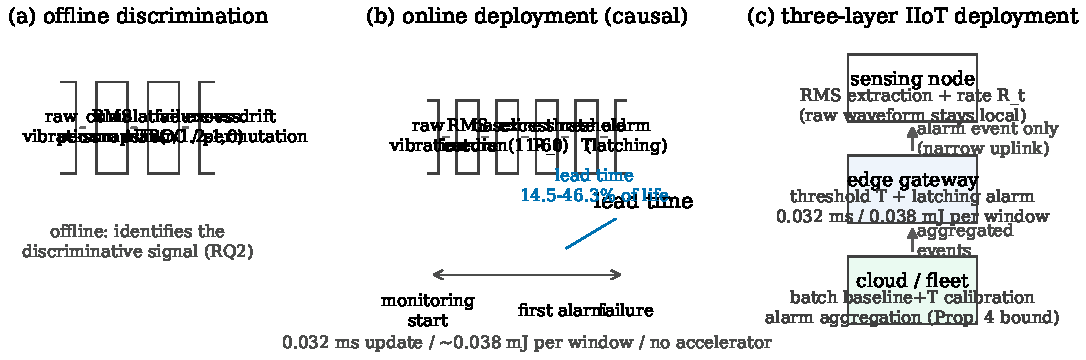
\includegraphics[width=\linewidth]{../figures/fig1_architecture.pdf}
\caption{Overall architecture: (a) the offline discrimination stage identifies the failure-versus-drift signal via the cumulative excess; (b) the online deployment stage is a causal six-step chain in which the RMS feature is baseline-calibrated and excess-rate--transformed before a single fixed threshold raises the alarm; (c) the three-layer IIoT deployment---sensing node (RMS + rate update), edge gateway (threshold + latching alarm), and cloud/fleet (batch calibration + aggregation)---with alarm-only uplink.}
\label{fig:arch}
\end{figure}

The middle panel of Fig.~\ref{fig:arch} collapses the online method into a six-step causal chain: raw vibration $\to$ RMS feature $f_i$ $\to$ baseline $b$ $\to$ excess rate $R_t$ $\to$ fixed threshold $T$ $\to$ latching alarm. Except for baseline estimation, every step is an incremental per-snapshot update that never accesses future data---the concrete meaning of ``causal and deployable.'' The right panel gives the three-layer IIoT deployment form (sensing node / edge gateway / cloud-fleet), developed in Section~\ref{sec:deploy}. The timeline also defines our lead-time convention: the alarm-to-failure interval as a percentage of life \eqref{eq:leadtime}, which avoids the incomparable cross-rig clocks (600\,s / 60\,s / 10\,s).

\subsection{Problem formalization and notation}
Consider one axis stream of one bearing. Let the $i$-th snapshot contain $m$ samples $x_{i,j}$ ($j=1,\dots,m$), with $N$ snapshots in total. The scalar health feature used by the online path is the per-snapshot RMS
\begin{equation}
f_i=\left(\frac{1}{m}\sum_{j=1}^{m}x_{i,j}^{2}\right)^{1/2}.
\label{eq:rms}
\end{equation}
The offline OOD benchmark additionally uses Pearson kurtosis, sample skewness, population variance, and peak-to-peak, computed from the same $x_{i,j}$ by their standard definitions and not numbered separately. The healthy baseline $b$ and relative amplitude $r_i$ are
\begin{equation}
b=\mathrm{median}\left\{f_i:11\le i\le60\right\},\qquad r_i=\frac{f_i}{b},
\label{eq:baseline}
\end{equation}
where the baseline window is snapshots 11--60 (discarding the first 10 run-in snapshots). The per-snapshot excess $e_i$ is the positive part of the relative amplitude above threshold $c$:
\begin{equation}
e_i=\max\left(r_i-c,\,0\right),\qquad c=1.2.
\label{eq:excess}
\end{equation}
Equations~\eqref{eq:rms}--\eqref{eq:excess} define the four basic quantities: $f_i$ the health feature, $b$ the healthy baseline, $r_i$ the normalized amplitude, and $e_i$ the per-snapshot excess. Table~\ref{tab:notation} collects all symbols.

\begin{table}[!t]
\caption{Notation used in this paper.}
\label{tab:notation}
\centering
\begin{tabular}{l l l}
\toprule
Symbol & Meaning & Type/range\\
\midrule
$x_{i,j}$ & $j$-th sample of the $i$-th snapshot & real\\
$m$ & samples per snapshot & positive integer\\
$f_i$ & RMS feature of the $i$-th snapshot \eqref{eq:rms} & nonnegative real\\
$i,t$ & snapshot index & positive integer\\
$N$ & total snapshots of the axis stream & positive integer\\
$b$ & early-life baseline \eqref{eq:baseline} & nonnegative real\\
$c$ & excess threshold (ratio), 1.2 & $c>1$\\
$r_i$ & relative amplitude \eqref{eq:baseline} & nonnegative real\\
$e_i$ & per-snapshot excess \eqref{eq:excess} & nonnegative real\\
$E_{\mathrm{cum}}$ & cumulative excess \eqref{eq:cumexcess} & nonnegative real\\
$S_t$ & excess running sum \eqref{eq:runningsum} & nonnegative real\\
$R_t$ & rate (time-averaged excess) \eqref{eq:rate} & nonnegative real\\
$T$ & alarm threshold (fixed scalar) \eqref{eq:threshold} & nonnegative real\\
$\tau$ & first alarm snapshot \eqref{eq:alarm} & $61,\dots,N$ or $\infty$\\
$L$ & lead time (\% of life) \eqref{eq:leadtime} & $0$--$100\%$\\
$\mathcal{C}$ & censored (healthy) bearing set & set\\
\bottomrule
\end{tabular}
\end{table}

\subsection{Data and feature representation}
Table~\ref{tab:datasets} summarizes the three public datasets (IMS~\cite{lee2007}, XJTU-SY~\cite{wang2020}, FEMTO/PRONOSTIA~\cite{nectoux2012}). SHA-256 of the raw archives are in the appendix; the features (RMS, Pearson kurtosis, sample skewness, population variance, peak-to-peak) are extracted by our scripts from raw signals per snapshot and per axis and compared row-by-row against the reference tables, with a maximum absolute error of about $10^{-14}$ (machine precision). The three datasets cover different sampling rates, snapshot intervals, and failure modes: IMS provides eight non-failed censored bearings, the key contrast for zero-false-alarm calibration and failure-versus-drift discrimination; XJTU-SY is all-failed with the most diverse failure modes; FEMTO has the shortest snapshot interval (10\,s), suited to validating lead-time temporal resolution. The online path uses only RMS; the other four features serve only the offline OOD benchmark. Data-count conventions: the three datasets contain 44 bearings in total; the online warning task requires $\ge70$ snapshots and evaluates 34 failed bearings (two of the 15 XJTU-SY bearings are excluded for having fewer than 70 snapshots); the degradation-OOD task requires $\ge120$ snapshots and evaluates 33 failed bearings (XJTU-SY uses 12).

In addition, Section~\ref{sec:rq1} uses two cross-condition fault-diagnosis benchmarks as diagnostic contrasts: CWRU (single bearing fault, speed drift only; source Loparo, Case Western Reserve University Bearing Data Center, benchmarked in~\cite{smith2015}) and the MCC5 gearbox compound-fault dataset (``Multi-mode fault diagnosis datasets of gearbox under variable working conditions,'' Mendeley Data, DOI 10.17632/p92gj2732w.1)~\cite{mcc5dataset}. The contrast baseline CASH v1.1 is a ``causal-anchor OOD scorer'' from our companion work, fully defined in Appendix~\ref{app:baselines} (input: per-window features; anchors: class anchors and class$\times$condition anchors; score: a conservative maximum of energy, anchor-reconstruction, and support residuals); in the main text it serves only as a cross-condition contrast, not as part of our online-warning contribution.

\begin{table}[!t]
\caption{Summary of the three public run-to-failure datasets.}
\label{tab:datasets}
\centering
\begin{tabular}{l c c c c c}
\toprule
Dataset & Bearings & Rate & Snapshot interval & Channels/axes & Failure modes\\
\midrule
NASA IMS & 12 (4 failed + 8 censored) & 20 kHz & 10 min (first 43 at 5 min) & 8/4 ch & inner/outer/roller\\
XJTU-SY & 15 (all failed) & 25.6 kHz & 1 min & horizontal + vertical & inner/outer/cage, etc.\\
FEMTO & 17 (6 learning + 11 full test) & 25.6 kHz & 10 s & horizontal + vertical & inner/outer/roller, etc.\\
\bottomrule
\end{tabular}
\end{table}

\subsection{Evaluation protocol}
For each bearing--axis stream we run a causal protocol: discard snapshots 1--10 (run-in); estimate the baseline $b$ from snapshots 11--60 \eqref{eq:baseline}; monitor online from snapshot 61; alarm by latching first-crossing \eqref{eq:alarm} with at least 30 monitored snapshots. The zero-false-alarm operating point is defined as $1.01\times$ the maximum rate over the healthy censored set \eqref{eq:threshold}---\emph{zero false alarms on the calibration set holds by construction, not by discovery}; what is reported is the detection rate and lead time at that point, with the false-alarm rate reported as 0/8 and its 95\% CI $[0,36.9\%]$. The $1.01$ factor in \eqref{eq:threshold} is a conservative margin rather than a fitted parameter: the sweep in Section~\ref{sec:robustness} shows factors $1.00/1.01/1.05/1.10$ all give 31/34, so the factor affects only the zero-false-alarm margin, not the detection rate. A bearing must have at least 70 snapshots to be evaluated. Sensitivity analysis (Section~\ref{sec:robustness}) shows the conclusions are stable to baseline windows 40/50/60, run-in 5/10/15, and minimum monitoring 10/30/60.

\subsection{Offline discriminative feature: cumulative excess (RQ2)}\label{sec:cumexcess}
\emph{Motivation.} RQ2 requires separating failure-bound degradation from benign drift under a zero-false-alarm constraint. The intuition is that the exceedances of a failed bearing accumulate persistently while benign drift is only occasional; integrating the ``part above $1.2\times$ baseline'' over the whole life decouples persistence from amplitude. \emph{Definition.} The cumulative excess is the whole-life sum of \eqref{eq:excess}:
\begin{equation}
E_{\mathrm{cum}}=\sum_{i=61}^{N}e_i=\sum_{i=61}^{N}\max\left(\frac{f_i}{b}-c,\,0\right).
\label{eq:cumexcess}
\end{equation}
Equation~\eqref{eq:cumexcess} (code identifier \texttt{auc\_above\_1p2x}) is a whole-life offline quantity that uses future snapshots and cannot be deployed online; it answers RQ2---on IMS the four failed and eight censored bearings are fully separated (AUROC 100, Section~\ref{sec:rq2})---and motivates the online form of Section~\ref{sec:rate}.

\subsection{Online rate-normalized detector (RQ3)}\label{sec:rate}
\emph{Motivation.} Turning the cumulative quantity into a time average makes the score independent of monitoring duration---the key to ``a single fixed threshold transfers across rigs,'' and the mechanism RQ4 tests. For $O(1)$ memory and $O(1)$ time we use a running-sum recursion:
\begin{equation}
S_t=S_{t-1}+e_t,\qquad S_{60}=0.
\label{eq:runningsum}
\end{equation}
The rate (time-averaged excess) is
\begin{equation}
R_t=\frac{S_t}{t-60}=\frac{1}{t-60}\sum_{i=61}^{t}e_i,\qquad t\ge61.
\label{eq:rate}
\end{equation}
The \emph{alarm rule} is a latching first crossing:
\begin{equation}
\tau=\min\left\{t\ge90:R_t>T\right\};
\label{eq:alarm}
\end{equation}
if the set in \eqref{eq:alarm} is empty then $\tau=\infty$ (no alarm); $t\ge90$ means at least 30 monitored snapshots. The \emph{threshold calibration} (one-time, offline, censored set $\mathcal{C}$ only) is
\begin{equation}
T=1.01\cdot\max_{k\in\mathcal{C}}\max_{t\ge61}R_t^{(k)}.
\label{eq:threshold}
\end{equation}
The \emph{lead time} (percentage of life) is
\begin{equation}
L=\frac{N-\tau}{N-60}\times100\%.
\label{eq:leadtime}
\end{equation}
\emph{Length invariance (the mechanism behind RQ4).} If the excess sequence $\{e_i\}$ is (weakly) stationary with $\E[e_i]=\mu$, then \eqref{eq:runningsum}--\eqref{eq:rate} give
\begin{equation}
\E[S_t]=\mu\,(t-60),\qquad \E[R_t]=\mu.
\label{eq:invariance}
\end{equation}
Equation~\eqref{eq:invariance} states that the expected running sum $S_t$ grows linearly with monitoring duration while the expected rate $R_t$ is constantly $\mu$. This formalizes why an unbounded accumulator must trigger a fixed threshold under benign drift while rate normalization is duration-independent (benign drift corresponds to $\mu>0$).

\subsection{Pseudocode and cost}
The online update is $O(1)$ time and $O(1)$ memory (keeping only the running sum $S_t$ and the count $t$).
\begin{algorithm}[!t]
\caption{Rate-normalized online early-warning detector (single axis).}
\label{alg:detector}
\begin{algorithmic}[1]
\REQUIRE $f[1..N]$ (single axis), $c=1.2$, run-in $=10$, $b_e=60$, $\mathrm{min\_mon}=30$, threshold $T$.
\ENSURE alarm snapshot $\tau$ or ``no alarm''.
\IF{$N < b_e+10$} \STATE \textbf{return} ``not evaluable'' \COMMENT{at least 70 snapshots}
\ENDIF
\STATE $b=\mathrm{median}(f[11..b_e])$ \COMMENT{snapshots 11--60}
\STATE $S=0$
\FOR{$t=b_e+1$ \TO $N$} \COMMENT{from snapshot 61}
\STATE $e=\max(f[t]/b-c,0)$
\STATE $S=S+e$
\STATE $R=S/(t-b_e)$ \COMMENT{time average}
\IF{$(t-b_e)\ge\mathrm{min\_mon}$ \AND $R>T$ \AND not alarmed}
\STATE $\tau=t$; alarm (latching); \textbf{break}
\ENDIF
\ENDFOR
\STATE \textbf{return} $\tau$ or ``no alarm''
\end{algorithmic}
\end{algorithm}
The threshold is calibrated one-time and offline from the censored bearings only, by \eqref{eq:threshold}. Edge cost (6-core Jetson Orin NX): RMS extraction 0.02--0.05 ms/window, detector update 0.032 ms/window, throughput about 18.3k windows/s, power delta 0.70 W, about 0.038 mJ/window, no accelerator.

\subsection{Online baselines (RQ4)}
The four comparison detectors use the same protocol and the same zero-false-alarm calibration \eqref{eq:threshold}, replacing only the score statistic. Shewhart uses the single-snapshot relative amplitude:
\begin{equation}
g_t^{\mathrm{Sh}}=r_t.
\label{eq:shewhart}
\end{equation}
EWMA uses exponentially smoothed excess ($\lambda=0.2$):
\begin{equation}
q_t=(1-\lambda)\,q_{t-1}+\lambda\,e_t,\qquad q_{60}=0,\quad\lambda=0.2.
\label{eq:ewma}
\end{equation}
CUSUM uses a reset cumulative excess with drift compensation $\delta$:
\begin{equation}
U_t=\max\left(0,\,U_{t-1}+e_t-\delta\right),\qquad U_{60}=0.
\label{eq:cusum}
\end{equation}
SPRT uses a reset cumulative Gaussian log-likelihood ratio:
\begin{equation}
\Lambda_t=\max\left(0,\,\Lambda_{t-1}+\ell_t\right),\qquad
\ell_t=\log\frac{\mathcal{N}\left(r_t;\mu_1,\sigma^2\right)}{\mathcal{N}\left(r_t;\mu_0,\sigma^2\right)}.
\label{eq:sprt}
\end{equation}
Equations~\eqref{eq:shewhart}--\eqref{eq:sprt} give the four baseline score statistics; $\mathcal{N}(r_t;\mu,\sigma^2)$ is a Gaussian density with mean $\mu$ and variance $\sigma^2$, $\mu_0,\mu_1$ are the healthy and degraded hypotheses, and $\sigma^2$ is estimated from the training segment. The offline degradation-OOD task additionally uses six unsupervised baselines---Mahalanobis, kNN-5, centroid distance, OC-SVM, isolation forest, and the RMS ratio (Section~\ref{sec:rq1}). The online warning additionally includes six modern baselines (Section~\ref{sec:rq4} and Appendix~\ref{app:baselines}): a window-level MLP autoencoder ($5\to3\to5$), a unidirectional LSTM autoencoder, Deep SVDD~\cite{ruff2018}, a causal Transformer autoencoder, TranAD~\cite{tuli2022tranad}, and a supervised RUL-thresholded baseline (unidirectional LSTM regression), all fed into the same causal protocol and zero-false-alarm calibration.

\subsection{Theoretical basis of rate normalization}\label{sec:theory}
The rate form of Section~\ref{sec:rate} is not an empirical choice but is forced by three constraints (causal, bounded, length-invariant). This section states four propositions (plus a weakly-dependent generalization in Proposition~5) that elevate the mechanism-level comparisons of Section~\ref{sec:results} to theoretical conclusions. We first clarify the positioning: Propositions~1--4 \emph{adapt} classical results (Birkhoff's ergodic theorem, Markov/Hoeffding inequalities, the Hoeffding supermartingale, and Ville's maximal inequality) to this detector; their value is in delivering the guarantee \emph{forms} needed for deployment (duration-independent pointwise and time-uniform false-alarm bounds), not in contributing new probability theory. Proposition~5 relaxes the i.i.d.\ assumption to weakly dependent excess and is a new step we add. Let $e_i$ \eqref{eq:excess}, $S_t$ \eqref{eq:runningsum}, and $R_t$ \eqref{eq:rate} be as defined.

\textbf{Proposition 1 (inevitable failure of unbounded accumulators).} If under healthy/benign drift the excess sequence $\{e_i\}$ is weakly stationary with $\E[e_i]=\mu>0$, then for any fixed threshold $T<\infty$, $S_t\to\infty$ a.s.; hence the fixed threshold is eventually crossed with probability one. \emph{Proof:} by the law of large numbers $S_t/(t-60)\to\mu>0$ a.s., so $S_t\to\infty$ a.s.; SPRT's accumulated log-likelihood ratio \eqref{eq:sprt} has, under drift mismatch, a positive-mean increment (nonnegative KL divergence), so it is a \emph{submartingale with positive drift} rather than a martingale, and the same conclusion holds. \emph{Corollary:} under a zero-false-alarm constraint an unbounded accumulator's threshold must grow with duration (order $t$), which then misses late real failures---the root cause of CUSUM 21/34 and SPRT 1/34 in Table~\ref{tab:detectors}.

\textbf{Proposition 2 (length invariance and scale equivariance of the rate).} Under Proposition~1's assumption, $\E[R_t]=\mu$ for all $t$ \eqref{eq:invariance}; $R_t$ is first-order homogeneous (equivariant to uniform scaling of the excess), so a threshold calibrated on dimensionless excess is transferable. \emph{Proof:} linearity gives $\E[R_t]=\E[S_t]/(t-60)=\mu$; homogeneity is immediate from $R_t=S_t/(t-60)$. Together with Proposition~3(b), the null distribution of $R_t$ collapses to $\mu$ as $t$ grows (self-normalized concentration)---the mechanism behind one fixed threshold across rigs.

\textbf{Proposition 3 (pointwise false-alarm bounds of the rate).} (a) Distribution-free: if $\E[e_i]=\mu$, Markov's inequality gives $\Prb(R_t>T)\le\mu/T$, independent of $t$, whereas $\Prb(S_t>T)\le(t-60)\mu/T$ diverges with $t$. (b) Concentration: if $e_i\in[0,M]$ i.i.d.\ and $\mu<T$, Hoeffding's inequality gives $\Prb(R_t>T)\le\mathrm{e}^{-2(t-60)(T-\mu)^2/M^2}\to0$. Both show that only the rate form has a time-independent (indeed decreasing) pointwise false-alarm bound under a fixed threshold, and the accumulator does not. Bound (a) is loose but distribution-free; (b) is tight when the excess is bounded; the threshold $T$ in \eqref{eq:threshold} can be interpreted as one level of this bound.

\textbf{Proposition 4 (anytime-valid time-uniform false-alarm bound of the rate).} If the excess $e_i$ is i.i.d.\ with $e_i\in[0,M]$ a.s.\ and $\E[e_i]=\mu<T$, then for any monitoring start $t_0\ge61$,
\begin{equation}
\Prb\left(\exists\,t\ge t_0:\ R_t\ge T\right)\le\mathrm{e}^{-2(t_0-60)(T-\mu)^2/M^2}.
\label{eq:anytime}
\end{equation}
\emph{Proof:} see Appendix~\ref{app:proof}. \emph{Remark:} Proposition~3 controls the false-alarm probability at a single time $t$, whereas Proposition~4 controls the union over the whole monitoring history---a genuinely anytime-valid bound. Its constant comes from the Hoeffding (boundedness) assumption; Bennett/Bernstein or e-value constructions can tighten it further, but it already suffices to prove that the rate form has false-alarm control that does not diverge with duration, which the accumulator (Proposition~1) lacks.

\textbf{Proposition 5 (pointwise false-alarm bound under weakly dependent drift).} If the excess sequence $e_i\in[0,M]$ a.s.\ with $\E[e_i]=\mu<T$ is $\varphi$-mixing with mixing coefficients $\varphi(k)\le\bar\varphi\,k^{-a}$ ($a>2$), then for the monitoring duration $n=t-60$ and all sufficiently large $n$,
\begin{equation}
\Prb\left(R_n>T\right)\le\mathrm{e}^{-\sqrt{n}(T-\mu)^2/(2M^2)}+\bar\varphi\,n^{\frac12-\frac a4}.
\label{eq:mixing}
\end{equation}
\emph{Proof:} see Appendix~\ref{app:proof} (blocking/coupling). \emph{Remark:} when $a>2$ this bound decays to zero in $n$, i.e., the rate form retains a duration-independent pointwise false-alarm control under a weaker-than-i.i.d.\ assumption, directly addressing the i.i.d.\ limitation acknowledged in Section~\ref{sec:limitations}; the anytime-valid (time-uniform) extension under $\varphi$-mixing requires a blockwise e-value construction and is left as future work.

\emph{Occupation-time characterization.} $e_t=\max(r_t-c,0)$ is the positive part of the occupation of the RMS process above the barrier $c$; $E_{\mathrm{cum}}$ \eqref{eq:cumexcess} is a discrete occupation sum, $R_t$ is an occupation ratio, and the alarm \eqref{eq:alarm} is the first crossing of a fixed level by that occupation ratio. The detector can thus be described uniformly as ``a drift-robust fixed-level test on the occupation time of the healthy process''; Fig.~\ref{fig:theory} gives the empirical instantiation.

\section{Experiments and Results}\label{sec:results}

Results are organized by RQ. All detections run under the frozen protocol (Section~\ref{sec:cumexcess}); features are self-extracted from raw signals; the online-warning detection rate is reported per bearing (any-axis alarm) and also per axis. Unless noted, the detection-rate denominator is the 34 failed bearings.

\subsection{Degradation OOD is easy, cross-condition fault OOD is benchmark-dependent (RQ1)}\label{sec:rq1}
\emph{Core finding.} Degradation OOD reaches 91.04 macro AUROC (easy); cross-condition fault OOD difficulty is benchmark-dependent---MCC5 compound-fault held-condition is only 49.9--53.8, whereas CWRU single-fault held-condition reaches 93.3--96.8, a gap of about 40 points.

Table~\ref{tab:ood} reports per-method and per-dataset detail: all six unsupervised baselines exceed 92.5 macro AUROC except the naive RMS ratio (73.3); FEMTO (86.13) is markedly worse than IMS (96.89) and XJTU-SY (96.05). Fig.~\ref{fig:twoproblems} contrasts the mechanism: the degradation-OOD score strengthens monotonically and moves away from its early-life baseline, so any distance detector finds it trivially, whereas the MCC5 cross-condition score distributions overlap heavily (AUROC 49.9--53.8) while the CWRU held-condition distributions remain separable (CASH v1.1 96.8, Mahalanobis 93.3).

\begin{figure}[!t]
\centering
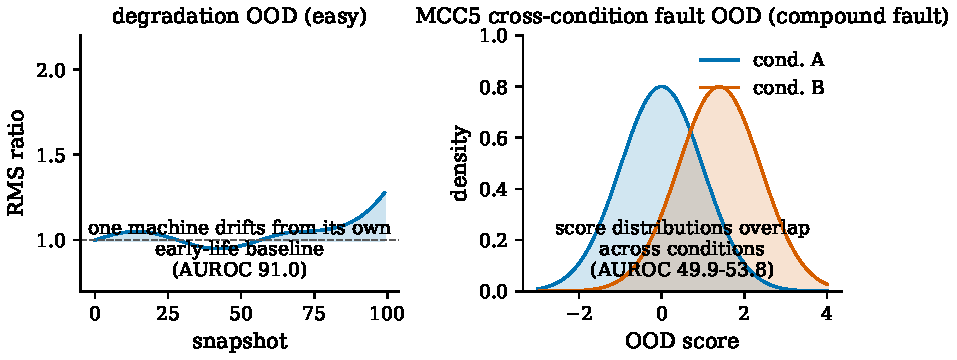
\includegraphics[width=\linewidth]{../figures/fig2_two_problems.pdf}
\caption{Mechanism contrast of the two OOD problems: left, degradation OOD (one machine drifting from its own early-life baseline, AUROC 91.0); right, MCC5 cross-condition fault OOD (score distributions overlap across conditions, AUROC 49.9--53.8).}
\label{fig:twoproblems}
\end{figure}

\begin{table}[!t]
\caption{Degradation-OOD benchmark and cross-condition contrasts: AUROC / FPR95 per method, per dataset, and cross-condition (33 failed bearings, single run; per-method values are per-stream means, per-dataset and macro values are per-bearing means); CASH v1.1 is a causal-anchor OOD scorer (cross-condition baseline).}
\label{tab:ood}
\centering
\begin{tabular}{l l c c}
\toprule
View & Item & AUROC & FPR95\\
\midrule
Method & kNN-5 distance & 96.54 & 10.47\\
Method & Isolation forest & 95.30 & 13.13\\
Method & Mahalanobis & 95.07 & 17.88\\
Method & Centroid distance & 93.00 & 23.94\\
Method & OC-SVM & 92.47 & 27.28\\
Method & RMS ratio & 73.32 & 46.13\\
Method & Reconstruction AE (5$\to$3$\to$5) & 95.62 & 15.56\\
Method & LSTM-AE (unidirectional, 3 seeds) & 95.28 & 14.27\\
Dataset & IMS (4 failed) & 96.89 & 9.75\\
Dataset & XJTU-SY (12) & 96.05 & 13.00\\
Dataset & FEMTO (17) & 86.13 & 33.20\\
Macro & 33 failed bearings & 91.04 & 23.01\\
Cross-cond.\ & CWRU held-condition CASH v1.1 & 96.77 & 5.01\\
Cross-cond.\ & CWRU held-condition Mahalanobis & 93.27 & 11.44\\
Cross-cond.\ & MCC5 held-condition Mahalanobis & 53.79 & 86.01\\
Cross-cond.\ & MCC5 held-condition CASH v1.1 & 49.86 & 91.92\\
\bottomrule
\end{tabular}
\end{table}

Observations from Table~\ref{tab:ood}: (i) kNN, isolation forest, Mahalanobis, centroid, OC-SVM, and the added reconstruction AE (95.6) and LSTM-AE (95.3) all exceed 92.5 AUROC; only the naive RMS ratio (73.3) is markedly low, so ``detecting deviation'' is not hard for mature and deep time-series baselines. (ii) FEMTO is markedly worse than the other two rigs. (iii) The macro FPR95 of 23.01 remains high and, together with the censored contrast (89.32 AUROC), shows the bottleneck is ``separating failure-bound degradation from benign drift at zero false alarms,'' not ``detecting deviation.'' The MLP-AE and LSTM-AE (3-seed per-bearing macro 94.90$\pm$0.21) both fail to beat the best simple baseline (kNN 96.5), further supporting ``degradation OOD is near-solved for simple baselines'' (aggregation note: Table~\ref{tab:ood}'s LSTM-AE 95.28 is a per-stream mean, whereas the 94.90$\pm$0.21 here is the 3-seed per-bearing macro mean---two different aggregation levels, not a contradiction); the macro 91.04 is the per-bearing mean of the six classical baselines and rises to about 91.7 when the AEs are added. The cross-condition rows directly give RQ1's second benchmark: CWRU (single bearing fault, speed drift only) held-condition OOD reaches 93.3--96.8, while MCC5 (gear/compound fault, speed+torque drift) is only 49.9--53.8---a gap of about 40 points---so cross-condition difficulty is set by drift type and fault type jointly, not by ``cross-condition is necessarily hard.''

The negative-transfer evidence of cross-condition threshold mismatch is Fig.~\ref{fig:negtransfer}: the same scores give held-condition ID false-positive rates of 2.8/52.7/79.2/27.7\% across the four MCC5 held conditions.

\begin{figure}[!t]
\centering
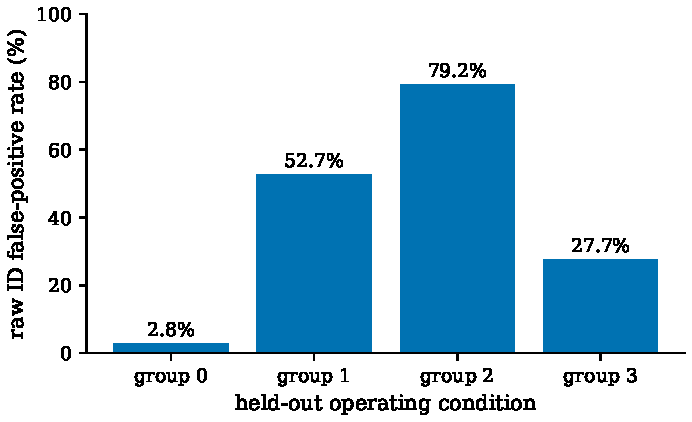
\includegraphics[width=\linewidth]{../figures/fig3_negative_transfer.pdf}
\caption{Negative-transfer evidence: held-condition in-distribution false-positive rates of the raw scores on the MCC5 cross-condition screening, up to 79.2\%.}
\label{fig:negtransfer}
\end{figure}

The four bars in Fig.~\ref{fig:negtransfer} do not sit at one level, meaning the threshold drifts sharply with condition and no single global threshold can suppress the false-positive rate across conditions. This contrasts with degradation OOD's per-machine baseline: the former needs cross-condition calibration, the latter only each machine's early-life baseline. \emph{Not claimed:} ``all degradation detection is easy and all cross-condition detection is hard''---the conclusion is limited to these three datasets and this protocol.

\subsection{Cumulative excess separates failure from drift (RQ2)}\label{sec:rq2}
\emph{Core finding.} The cumulative excess $E_{\mathrm{cum}}$ \eqref{eq:cumexcess} fully separates the four failed from the eight censored IMS bearings (AUROC 100, FPR95 0, exact permutation $p=1/495$, the minimum attainable for a $4$-vs-$8$ full separation), with failed median 0.099 vs.\ censored 0.019 (median ratio $\approx5.2$); the leave-one-bearing AUROC stays 100 (12/12), and the bootstrap 20{,}000-times CI degenerates to $[100,100]$. This result is read as \emph{mechanistic evidence}---it proves the ``persistence'' signal exists---rather than as a performance claim on $n=4$.

Fig.~\ref{fig:faildrift} shows the mechanism on real trajectories: the failed bearing (inner race, test1 B3) and the censored bearing (test1 B1) both cross the $1.2\times$ line many times, so ``exceeded or not'' alone cannot separate them; in the lower panel the failed bearing's rate $R_t$ grows persistently past the threshold $T$ while the censored bearing stays below.

\begin{figure}[!t]
\centering
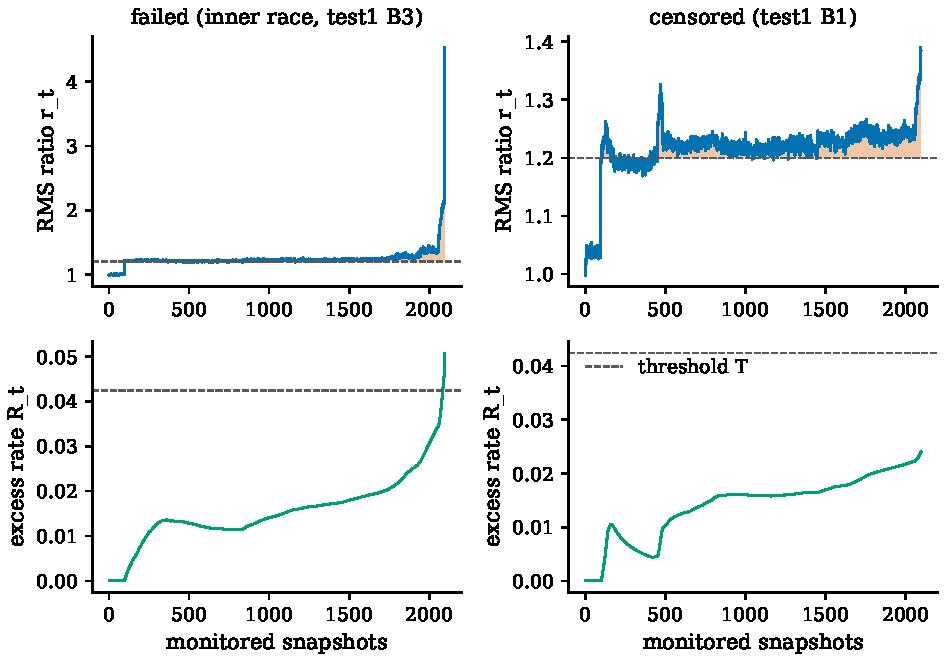
\includegraphics[width=\linewidth]{../figures/fig4_failure_vs_drift.pdf}
\caption{The ``persistence $>$ amplitude'' mechanism on real IMS trajectories: the failed bearing persistently exceeds $1.2\times$ baseline and accumulates excess, while the censored bearing only exceeds occasionally; lower panels show the corresponding excess rate $R_t$ and threshold $T$.}
\label{fig:faildrift}
\end{figure}

\emph{Not claimed:} $n=4$; the significance is real (the $p$-value is already the minimum attainable) but generalizability is unproven, so this is not used as the headline number.

\subsection{Rate-normalized detector and lead time (RQ3)}\label{sec:rq3}
\emph{Core finding.} At the zero-false-alarm operating point ($T=0.0424$) it detects 31/34 (95\% CI 76.3--98.1\%), false alarms 0/8 (95\% CI 0--36.9\%); median lead times are 14.5\%/46.3\%/36.0\% of life (about 23.2 h / 1.1 h / 1.3 h); per-axis 58/66 (87.9\%) vs.\ per-bearing 91.2\%. Cross-dataset heterogeneity is stated explicitly: IMS (4/4) and XJTU-SY (13/13) hit a 100\% ceiling, and FEMTO (14/17 = 82.4\%) is the only genuine cross-rig generalization test. The three FEMTO misses' ``low-amplitude degradation'' is data-supported (Appendix~\ref{app:baselines}): the missed bearings have median max RMS ratio 4.15 and median cumulative excess 62.3, versus 7.82 and 306.5 for the detected bearings---the misses are low-amplitude and low-persistence jointly, not random failures.

Fig.~\ref{fig:opcurve}'s $c$-sweep shows that $c=1.2$ is the ``31/34 detection + 28.8\% median lead time'' trade-off point; larger $c$ (1.55 and 1.8--2.0) reaches 32/34 (94.1\%), but the lead time declines overall as $c$ grows, reaching only 17.5\% at $c=2.0$ (about 11 points lost relative to $c=1.2$), whereas $c=1.55$ loses only about 3 points.

\begin{figure}[!t]
\centering
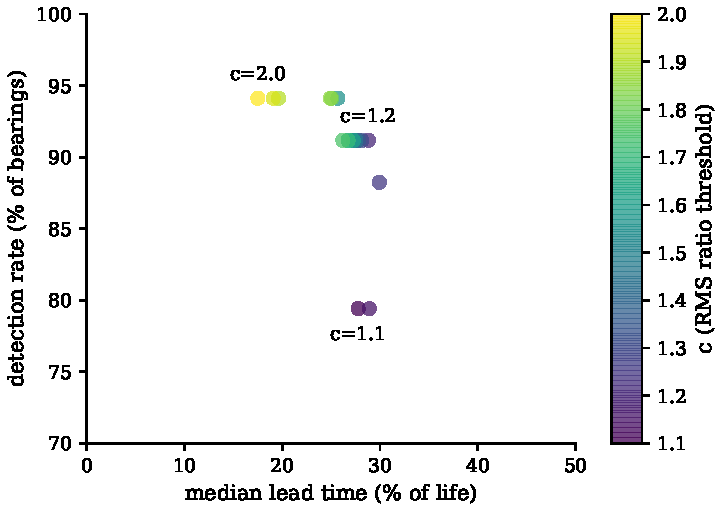
\includegraphics[width=\linewidth]{../figures/fig5_operating_curve.pdf}
\caption{Operating curve over the threshold $c$: every $c$ is re-calibrated to zero false alarms on the censored set, dots are per-bearing detection rate vs.\ median lead time, color encodes $c$.}
\label{fig:opcurve}
\end{figure}

Each $c$ in Fig.~\ref{fig:opcurve} independently re-computes the zero-false-alarm threshold on the censored set (zero false alarms holds by construction), so the curve is non-monotonic and is the true ``detection--lead-time'' trade-off; raising $c$ can at most move detection from 31/34 to 32/34 while pushing lead time from 28.8\% down to 17.5\% (a marginal gain of one bearing at a cost of about 11 points of lead time), so $c=1.2$ is retained; this sweep supports $c=1.2$ independently of the external protocol~\cite{hora_submitted,hora_unpublished}. \emph{Not claimed:} zero false alarms is by construction, not discovered. To turn the ``only 8 IMS censored bearings'' weakness into a measurable number, we add a cross-rig false-alarm proxy (Appendix~\ref{app:baselines}): taking the first 150 snapshots of each XJTU-SY/FEMTO bearing as an early-life pseudo-health segment (these bearings eventually fail but are healthy in the segment), the exceedance rate against $T=0.0424$ is a point estimate of 18.5\% per axis (10 of 54 axes; 95\% CI 9.3--31.4\%; XJTU-SY 30\%, FEMTO 11.8\%) and about 22\% per bearing---an estimate of pseudo-health segments, not a strict upper bound. The threshold therefore transfers across rigs only at a measurable residual cost, which we disclose rather than hide.

\subsection{Comparison with classical and modern baselines (RQ4)}\label{sec:rq4}
\begin{figure}[!t]
\centering
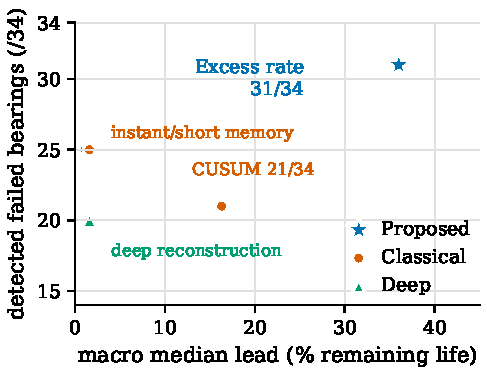
\includegraphics[width=\linewidth]{../figures/fig9_method_tradeoff.pdf}
\caption{Detection--lead-time trade-off under the same causal protocol and zero-false-alarm calibration. The horizontal coordinate is the median of the three per-dataset median lead times. SPRT is omitted because it detects only one failed bearing, and seed-unstable Deep SVDD/RUL-LSTM are omitted because they have no meaningful aggregate lead time. Among the stable baselines shown, the excess-rate detector is Pareto-dominant: it provides both the largest detection count and the longest macro median lead.}
\label{fig:tradeoff}
\end{figure}

\emph{Core finding.} Under the same protocol and zero-false-alarm calibration, excess rate 31/34 $>$ Shewhart 25 $\approx$ EWMA 25 $>$ CUSUM 21 $>$ SPRT 1, and it is well above all four window-level deep reconstruction baselines (MLP-AE, LSTM-AE, Transformer-AE, TranAD, each 20/34) and the supervised RUL-thresholded baseline (median 6/34) (Table~\ref{tab:detectors}; baseline statistics in \eqref{eq:shewhart}--\eqref{eq:sprt} and Appendix~\ref{app:baselines}).

\begin{table}[!t]
\caption{Per-dataset detection count and median lead time of the online detectors under zero-false-alarm calibration (34 failed + 8 censored).}
\label{tab:detectors}
\centering
\begin{tabular}{l c c c c c c}
\toprule
Detector & Det.\ (/34) & IMS & XJTU-SY & FEMTO & Median lead (\%) & Zero-FA thr.\\
\midrule
Excess rate (ours) & 31 & 4/4 & 13/13 & 14/17 & 14.5 / 46.3 / 36.0 & 0.042\\
Shewhart & 25 & 2/4 & 11/13 & 12/17 & 0.7 / 6.8 / 1.1 & 5.69\\
EWMA & 25 & 2/4 & 11/13 & 12/17 & 0.6 / 6.4 / 1.6 & 3.53\\
CUSUM & 21 & 3/4 & 9/13 & 9/17 & 4.4 / 16.3 / 27.3 & 169.5\\
SPRT & 1 & 1/4 & 0/13 & 0/17 & 37.8$^{\ddagger}$ / --- / --- & $1.13\times10^{6}$\\
MLP-AE (window) & 20 & 3/4 & 9/13 & 8/17 & 0.2 / 1.2 / 25.1 & $2.4\times10^{5}$\\
LSTM-AE (unidir.) & 20 & 3/4 & 9/13 & 8/17 & 0.2 / 1.2 / 25.1 & $2.4\times10^{5}$\\
Transformer-AE (causal) & 20 & 3/4 & 9/13 & 8/17 & 0.2 / 1.6 / 25.7 & $2.4\times10^{5}$\\
TranAD (causal) & 20 & 3/4 & 9/13 & 8/17 & 0.2 / 1.6 / 25.7 & $2.4\times10^{5}$\\
Deep SVDD (3-seed median) & 2 & 1/4 & 1/13 & 0/17 & --- & 0.26\\
RUL-LSTM (supervised, 3-seed median) & 6 & 1/4 & 4/13 & 5/17 & --- & 0.13\\
\bottomrule
\end{tabular}
\par\vspace{2pt}
{\footnotesize Zero-false-alarm thresholds are calibrated on the 8 IMS censored bearings; McNemar/Holm significance is in the text. $^{\ddagger}$ SPRT's 37.8\% lead is based on a single sample (IMS 1/4) and carries no statistical meaning; the remaining SPRT lead times are empty. The four reconstruction baselines (MLP-AE/LSTM-AE/Transformer-AE/TranAD) all have a threshold ($\approx2.4\times10^{5}$) dominated by one drifted window of censored bearing test3\_b4; Deep SVDD (1/22/2 across seeds) and RUL-LSTM (theta 0.13 to $-0.03$) are seed-unstable, so their medians are reported.}
\end{table}

Observations: Shewhart and EWMA detect a tolerable 25 but with near-zero lead time (0.6--6.8\%), of no operational value for predictive maintenance; CUSUM and SPRT are nearly or fully destroyed (21/34 and 1/34) by integrating benign drift and the consequently raised zero-false-alarm threshold; SPRT's 1/34 is not an implementation artifact but the inevitable outcome of its misspecified Gaussian null, under which the log-likelihood ratio drifts positively under benign drift (Proposition~1, Appendix~\ref{app:proof}). The four window-level deep reconstruction baselines (MLP-AE/LSTM-AE/Transformer-AE/TranAD) all detect exactly 20/34 with the identical 3/9/8 per-dataset split: their per-window reconstruction error is an \emph{unbounded magnitude quantity} dominated by the window's distance from the healthy training support rather than by learned fault structure, and a drifted window of the censored bearing test3\_b4 (RMS ratio 5.63) raises the zero-false-alarm threshold to about $2.4\times10^{5}$, suppressing detection---the same benign-drift-threshold mechanism as CUSUM/SPRT, but realized through per-window magnitude rather than accumulation. Deep SVDD is unstable when trained on only about 50 healthy windows (1--22/34 across seeds). The supervised RUL-thresholded baseline is trained in-sample on all failed bearings and evaluated on the same bearings---an upper-bound (favorable) treatment for a baseline---yet it remains seed-unstable (median 6/34, best 29/34): it must extrapolate remaining life for the never-failing censored bearings, and that extrapolation swings between positive and negative values across seeds, collapsing the threshold. Paired McNemar exact tests (34 failed bearings): vs.\ CUSUM discordant pairs 10/0 ($p=0.002$, Holm $p=0.006$), vs.\ SPRT 30/0 ($p<0.001$, Holm $p<0.001$) are significant; vs.\ Shewhart/EWMA 6/0 each (raw $p=0.031$, Holm $p=0.063$) is nominally significant but does not survive four-way correction.

\emph{Normalized-accumulator fairness check.} The rate $R_t=S_t/(t-60)$ is, by construction, a zero-drift-compensation, no-reset, time-normalized CUSUM. To rule out ``beating an unbounded strawman,'' we add, under the same protocol, a normalized reset CUSUM ($U_t=\max(0,U_{t-1}+e_t-\delta)$ divided by $t-60$, $\delta\in\{0,0.005,0.01,\hat\mu\}$, with $\hat\mu=0.0153$ the censored mean drift) and a normalized SPRT ($\Lambda_t/(t-60)$): $\delta=0$ reduces to the rate (31/34, a self-check); $\delta=0.005$ gives 31/34; $\delta=0.01$ and $\delta=\hat\mu$ drop to 30/34; normalized SPRT gives only 4/34. Within the normalized-accumulator family, zero drift compensation and no reset is therefore optimal---drift compensation must estimate $\mu$ from only eight censored bearings, and the estimation error lowers sensitivity; normalization cannot repair SPRT's misspecified Gaussian null (Appendix~\ref{app:baselines}).

Fig.~\ref{fig:tradeoff} condenses the deployment-relevant comparison: the excess-rate detector is the only displayed method that combines high detection with substantial lead time. Fig.~\ref{fig:ratecum} visualizes the failure mechanism of unbounded accumulators: on censored bearings the CUSUM/SPRT scores climb monotonically with monitoring duration, and after normalizing each score by its own zero-false-alarm threshold, only the rate crosses the normalized line 1.

\begin{figure}[!t]
\centering
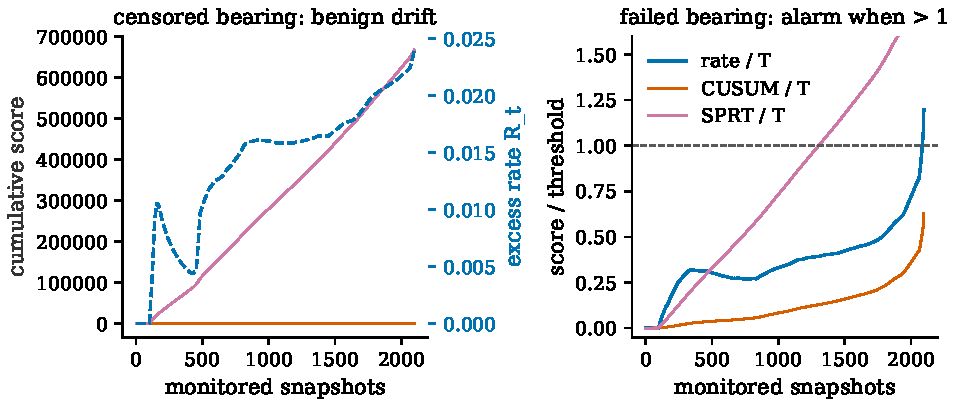
\includegraphics[width=\linewidth]{../figures/fig6_rate_vs_cumulative.pdf}
\caption{What rate normalization buys: (a) benign drift of censored bearings is integrated persistently by CUSUM/SPRT while the rate stays flat; (b) on failed bearings, after normalizing by each score's zero-false-alarm threshold, only the rate crosses 1.}
\label{fig:ratecum}
\end{figure}

\emph{Not claimed:} the detection-count difference between Shewhart/EWMA and the rate does not survive correction; our advantage over them rests mainly on lead time (qualitative) and on the ``unbounded accumulator fails'' result (significant).

\subsection{Ablation and negative results}
\emph{Per-feature ablation (Table~\ref{tab:features}).} Under the same protocol and zero-false-alarm calibration, changing only the scalar feature: RMS 31/34 is best, variance 29/34 second, kurtosis 17/34 worst.

\begin{table}[!t]
\caption{Per-feature ablation (34 failed bearings, same protocol and zero-false-alarm calibration, changing only the scalar feature).}
\label{tab:features}
\centering
\begin{tabular}{l c c c}
\toprule
Feature & Det.\ (/34) & Detection rate (\%) & Median lead (\%) \\
\midrule
RMS (ours) & 31 & 91.2 & 28.8\\
Variance & 29 & 85.3 & 28.3\\
Skewness & 26 & 76.5 & 94.7$^{\dagger}$\\
Peak-to-peak & 24 & 70.6 & 51.6\\
Pearson kurtosis & 17 & 50.0 & 67.9$^{\dagger}$\\
\bottomrule
\multicolumn{4}{l}{\footnotesize $^{\dagger}$ The early-life median of skewness/kurtosis is near zero, so the $1.2\times$ ratio rule is ill-posed for them; their lead-time numbers are not interpreted---the detection rate is the primary ablation output.}
\end{tabular}
\end{table}

\emph{Spectral-feature ablation (negative).} On IMS, envelope kurtosis and fault-frequency envelope ratio give failure-versus-drift AUROC 96.9 / 78.1 and zero-false-alarm detections 2/4 each, not better than RMS (100 / 4/4). \emph{Negative transfer (negative).} On MCC5, requiring $k\ge2$ consecutive exceedances only lowers the ID false-positive rate from about 3\% to about 1\% while delaying E2/E3/E5 alarms by $>730$ windows. \emph{Not claimed:} these negative results do not negate spectral features elsewhere; they only show that for these three rigs the energy (RMS) rise is already a robust early signal.

\emph{Dual-scale activation mechanism probe.} To distinguish historical persistence from recent activation, we additionally compute the causal mean $A_t^{(3)}$ of excess over three monitoring snapshots and independently apply the same 1.01 zero-false-alarm calibration on the IMS censored set. The recent rate alone reaches only 27/34 with 2.94\% median lead, so transient activation cannot replace accumulation; allowing $R_t$ or $A_t^{(3)}$ to cross its calibrated threshold on any axis gives 32/34 and 0/8 false alarms, adding one FEMTO bearing, but the gain disappears when the window increases from three to five snapshots. We use this result as a mechanism probe rather than a headline: historical rate remains the primary signal, and the remaining FEMTO failures still mark the abrupt/low-early-energy boundary.

\emph{Hierarchical cross-axis persistence (exploratory).} The remaining FEMTO misses are not low-amplitude; they show late simultaneous activation on two axes, whereas IMS censored streams contain isolated one-axis transients. Let $A_{k,t}^{(10)}$ denote the ten-snapshot recent excess mean of axis $k$ and $J_t=\mathrm{secondmax}_k A_{k,t}^{(10)}$. By construction, $J_t$ can cross its threshold only when at least two axes corroborate recent activation. The hierarchical rule alarms when any axis has $R_t>T_R$ or $J_t>T_J$. Historical rate, cross-axis rate, and the hierarchy detect 31/34, 32/34, and 34/34, all with 0/8 IMS false alarms; the hierarchy has 28.64\% median lead, and its three additional FEMTO detections occur 0.75\%, 33.46\%, and 1.01\% of life before failure. The hierarchy remains 34/34 for windows 5--100 and margins 1.00--1.20. On 27 early-life pseudo-health bearings, the respective bearing-level false-alarm counts are 6/27, 4/27, and 6/27, so the hierarchy does not worsen the cross-rig proxy. Nevertheless, the three additions have no reversals (exact McNemar $p=0.25$), leave-one-censored-out calibration gives 2/8 held-out false alarms, and only two multi-axis IMS censored bearings calibrate $T_J$. We therefore report this as a mechanism-driven post-hoc extension, not a replacement for the 31/34 headline.

\subsection{Edge cost, robustness, and protocol sensitivity}\label{sec:robustness}
\emph{Core finding.} The detector update takes 0.032 ms/window; the full RMS-extraction-plus-update pipeline takes about 0.038 mJ/window (0.70 W load delta at about 18.3k windows/s), no accelerator (Jetson Orin NX). The two figures are reported separately: 0.032 ms is the pure threshold update, while 0.038 mJ is the energy of the whole overlapping RMS-plus-update pipeline per window; they are not two units of one operation. Robustness (threshold $T=0.0424$ fixed, not re-tuned under perturbation): with 1--10\%-of-baseline zero-mean Gaussian noise on RMS the detection stays 31/34; in the per-bearing per-axis dropout trials (68 runs) the worst is 30/34 and the median 31/34. A causal RMS-feature quantization stress test, using a fixed $[0,8b]$ range set by the already-observed baseline $b$ and no future sample, preserves 31/34 detections and 0/8 false alarms at 8--24 bits; at 8 bits the median lead is 28.46\% versus 28.82\% at full precision. This is a feature-domain result, not a raw-ADC validation. Protocol sensitivity: the detector ordering (excess-rate 31 $>$ Shewhart 25--26 $>$ EWMA 25 $>$ CUSUM 21 $>$ SPRT 1) is invariant to baseline windows 40/50/60; 31/34 is invariant to run-in 5/10/15 and min-monitor 10/30 (min$=$60 gives 30/34). The threshold-margin factor (the $1.01$ in \eqref{eq:threshold}) swept over $\{1.00,1.01,1.05,1.10\}$ always gives 31/34, proving the factor sets only the zero-false-alarm margin, not the detection rate (Appendix~\ref{app:baselines}). The EWMA $\lambda$ swept over $\{0.05,0.1,0.2,0.3,0.5\}$ gives 23/25/25/26/28 (best 28, still below 31); the SPRT alternative mean swept over $\{1.05,1.1,1.2,1.3,1.5\}$ gives 1/1/1/3/6 (best 6, far below 31)---neither sweep changes the Section~\ref{sec:rq4} ranking, ruling out an unfavorable-tuning explanation (Appendix~\ref{app:baselines}).

\subsection{IIoT deployment analysis}\label{sec:deploy}
The rate-normalized detector is an $O(1)$-memory, $O(1)$-time, accelerator-free scalar detector whose deployment form is three-layered: \emph{sensing node} (RMS extraction + per-window rate update) $\to$ \emph{edge gateway} (threshold comparison, latching event, local baseline/threshold) $\to$ \emph{cloud/fleet management} (one-time baseline/threshold batch calibration and alarm aggregation). On the data path, raw waveforms never leave the node and only alarm events travel uplink, matching the massive-node, narrow-uplink constraints of IIoT; Proposition~4 gives a duration-independent time-uniform false-alarm bound that makes every uplinked alarm statistically trustworthy. This three-layer form is annotated in Fig.~\ref{fig:arch}, and it answers the ``removing the edge constraint leaves the evaluation intact'' concern: energy, bandwidth, and fleet scale are not evaluation appendices but the constraints that drive the design choice of rate normalization ($O(1)$, duration-independent, provably bounded false alarms).

Energy measurement protocol (Jetson Orin NX, 6 cores): jtop/VDD power-rail sampling, 5\,s idle warm-up baseline, 60\,s sustained-loop throughput measurement, five repetitions averaged; the 18{,}266 windows/s throughput corresponds to the full pipeline on XJTU-length windows (32{,}768 samples). Measured idle 5{,}834 mW, load 6{,}533 mW, load delta 698.9 mW, hence 0.0383 mJ per full-pipeline window (698.9 mW $\div$ 18{,}266 windows/s). At the shortest 10\,s snapshot interval the detector's yearly energy is on the order of a hundred joules, and with event-driven reporting it supports long-term deployment under battery or energy-harvesting power. At the fleet level, nodes run independently and the center performs only one-time batch calibration and aggregation, so the system scales horizontally. Risks: the zero-false-alarm threshold depends on healthy censored calibration, and a new rig without healthy-running data cannot guarantee the false-alarm rate (the cross-rig proxy of Section~\ref{sec:rq3} gives about 18\% per axis); very-fast failure and low-amplitude degradation are two known blind spots.

\subsection{Fleet-scale false-alarm budget}
Per-machine zero-false-alarm calibration does not compose across a fleet. Aggregating the cross-rig per-axis false-alarm rate $p=0.185$ (per 150-snapshot early-life segment) as independent Bernoulli trials (Fig.~\ref{fig:fleet}): one machine with two axes raises at least one false alarm in an epoch with probability $1-(1-p)^2\approx33.6\%$; this reaches 98.3\% at 10 machines and saturates to $100\%$ at 100 machines (37 expected false alarms per epoch, 370 at 1000). The independence assumption is bootstrap-checked (Appendix~\ref{app:baselines}): only 2 of the 54 pseudo-health axes belong to bearings with mixed-axis alarms, so alarm events cluster within bearings and the axis-independent model is conservative; under a bearing-clustered rate $p=0.222$, a 100-machine fleet has about 22 false alarms per epoch, with a bootstrap 95\% CI of $[11,67]$---the order of magnitude and the conclusion (fleet false alarms are unavoidable in bulk) are unchanged. To hold the fleet-wide ``at least one false alarm per epoch'' probability below 5\%, the per-axis rate must be tightened to roughly $\alpha/(Mk)$, i.e., about 0.0256\% for 100 machines and 2 axes---a $\approx720\times$ tightening relative to 18.5\% that cannot be achieved by raising one threshold without losing detection. This agrees with the union-bound composition of Proposition~4: bounding the per-axis anytime-valid bound over $Mk$ axes, the data-driven excess bound $M=4.43$ makes the guarantee essentially non-decaying at realistic horizons (about 0.99 per axis at $n_0=30$), so the theory provides a \emph{form} guarantee (false-alarm probability does not diverge with monitoring duration) while fleet-level numeric control can only come from empirical calibration and fleet-level alarm management (multi-axis confirmation, event aggregation, hierarchical thresholds).

\begin{figure}[!t]
\centering
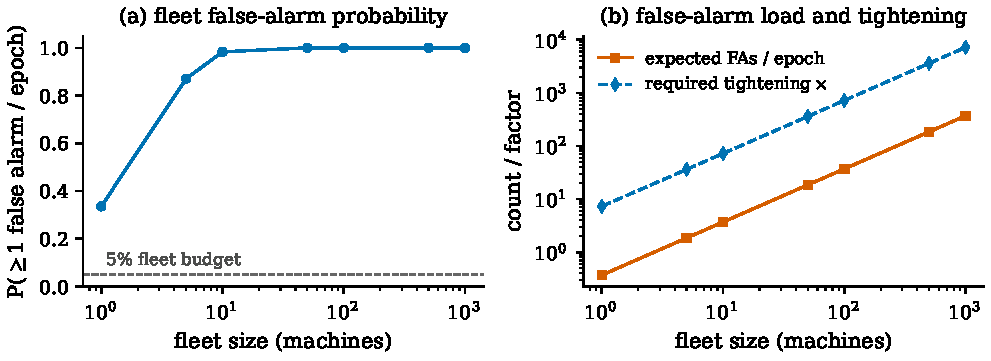
\includegraphics[width=\linewidth]{../figures/fig8_fleet_false_alarm.pdf}
\caption{Fleet-scale false-alarm budget: (a) the fleet-wide ``at least one false alarm per epoch'' probability saturates to one as fleet size grows; (b) expected false alarms per epoch grow linearly with fleet size, and the required per-axis tightening to keep a 5\% fleet budget grows super-linearly (log scale).}
\label{fig:fleet}
\end{figure}

\begin{figure}[!t]
\centering
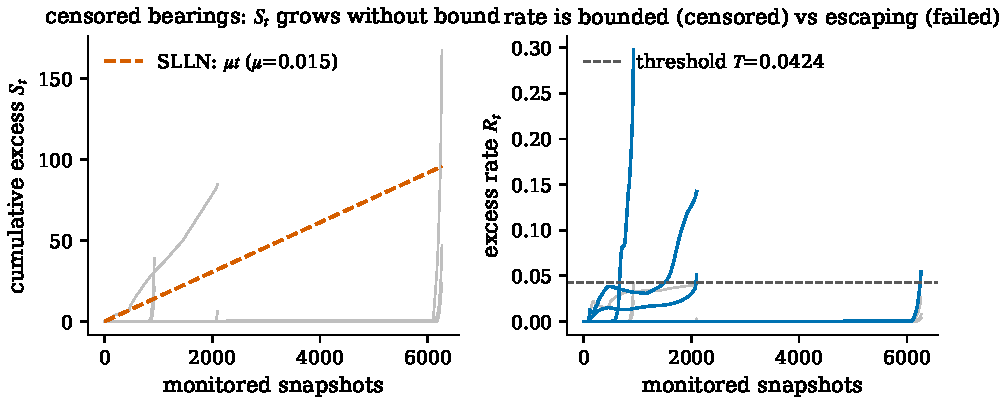
\includegraphics[width=\linewidth]{../figures/fig7_rate_length_invariance.pdf}
\caption{Data-side validation of Propositions 1--4: (a) the cumulative excess $S_t$ of the eight censored bearings grows linearly with monitoring duration, matching the $\mu t$ reference ($\mu=0.0153$, the per-snapshot excess averaged over the censored bearings), so any fixed threshold is eventually crossed; (b) the rate $R_t$ of the same bearings is bounded and converges, and only failed bearings cross the fixed threshold $T=0.0424$.}
\label{fig:theory}
\end{figure}

\section{Discussion and Limitations}\label{sec:discussion}

\subsection{Answers to the research questions}
\textbf{RQ1.} The same unsupervised methods reach 91.04 macro AUROC on degradation OOD; cross-condition fault OOD difficulty is benchmark-dependent---MCC5 compound-fault held-condition is 49.9--53.8 (its held-condition ID false-positive rates drift to 2.8/52.7/79.2/27.7\%) while CWRU single-fault held-condition reaches 93.3--96.8. This supports the diagnosis contribution and sharpens the conclusion to ``cross-condition difficulty is set by drift type and fault type jointly,'' not ``cross-condition is necessarily hard.'' Evidence strength: \emph{supported}, but limited to these benchmarks and this protocol; MCC5's near-chance result does not extend to single-bearing-fault/RPM-drift (CWRU is a counterexample), and degradation OOD's easiness rests on three rigs only.

\textbf{RQ2.} The cumulative excess $E_{\mathrm{cum}}$ \eqref{eq:cumexcess} fully separates IMS 4 failed vs.\ 8 censored (AUROC 100, FPR95 0, exact permutation $p=1/495$, median ratio $0.099/0.019\approx5.2$). This supports the method contribution and is read as mechanistic evidence. Evidence strength: \emph{partially supported}---the significance is real but $n=4$ failed, generalizability unproven; low-amplitude degradation (three FEMTO misses) is its known failure mode.

\textbf{RQ3.} The rate-normalized form detects 31/34 (95\% CI 76.3--98.1\%) at the zero-false-alarm operating point, with lead times 14.5\%/46.3\%/36.0\% of life, a 0.032 ms/window update, and about 0.038 mJ/window for the full pipeline. This supports the method and system contributions. Evidence strength: \emph{supported}, but ``zero false alarm'' is by construction and the cross-rig false-alarm proxy point estimate is about 18.5\% per axis (10/54; 95\% CI 9.3--31.4\%, Appendix~\ref{app:baselines}); this wording must be preserved.

\textbf{RQ4.} Under the same protocol and calibration, 31/34 $>$ Shewhart 25 $\approx$ EWMA 25 $>$ CUSUM 21 $>$ SPRT 1, and above all window-level deep reconstruction baselines (MLP-AE/LSTM-AE/Transformer-AE/TranAD) at 20/34 and the supervised RUL-thresholded baseline (median 6/34); McNemar is significant against CUSUM (Holm $p=0.006$) and SPRT (Holm $p<0.001$) but not against Shewhart/EWMA (Holm $p=0.063$). The EWMA/SPRT parameter sweeps (Appendix~\ref{app:baselines}) do not change the ranking. This supports the theory and method contributions. Evidence strength: \emph{partially supported}---the necessity of the rate over unbounded accumulators is significant, and its edge over deep reconstruction baselines rests on the benign-drift threshold mechanism; its detection-count edge over instantaneous/short-memory rules does not survive correction, and the advantage is mainly lead time (0.6--6.8\% vs.\ 14.5--46.3\%).

\subsection{Three-layer mechanism and evidence boundary}
The evidence chain is read in three steps: (i) mechanism---persistence rather than instantaneous amplitude separates failure-bound degradation from benign drift; (ii) statistics---the zero-false-alarm operating point is empirical, while the theoretical bounds require additional independence or mixing assumptions; and (iii) engineering---edge feasibility must be evaluated jointly with fleet-scale false-alarm cost. The detailed evidence is as follows.
\emph{Directly data-supported:} persistence $>$ amplitude---the cumulative excess perfectly separates $n=12$ (Figs.~\ref{fig:faildrift},~\ref{fig:theory}); the recent rate alone reaches 27/34 with only 2.94\% median lead, whereas the historical rate reaches 31/34 with 28.8\% lead; the cross-axis layer alone covers all 17 FEMTO failures but misses two IMS failures, showing that corroborated recent activation and long-history persistence are complementary rather than redundant; unbounded accumulators integrate benign drift and invalidate the fixed threshold (CUSUM/SPRT significantly worse, Fig.~\ref{fig:ratecum}, Proposition~1); window-level AE/LSTM-AE reconstruction error is threshold-inflated by a censored drift window (Table~\ref{tab:detectors}, 20/34). \emph{Physical interpretation (analogy, not a fitted damage law):} wear and fatigue cracking are commonly represented as nonnegative, approximately monotone damage accumulation; $e_i$ serves as a broadband energy proxy for such accumulation, and rate normalization estimates its coarse-grained damage rate. We do not estimate wear coefficients or crack length and do not claim that $e_i$ equals physical damage. \emph{Theoretically supported:} the rate form's length invariance and time-independent/time-uniform false-alarm bounds are given by Propositions~2--4; Proposition~5 extends the pointwise bound to $\varphi$-mixing (weakly dependent) excess. \emph{Ablation/control supported:} rate normalization is the key design choice (same-protocol 31 vs.\ 21/1 vs.\ 20); RMS is the robust feature (per-feature ablation 31/34 best, spectral features not better); within the normalized-accumulator family zero drift compensation is optimal (31 vs.\ 30/4, Appendix~\ref{app:baselines}). \emph{Assumption check (negative result):} the censored excess autocorrelation at lags 1/5/20 is 0.92/0.90/0.80 with fitted power-law exponent $a\approx0.18$, i.e., the excess is near-unit-root persistent and satisfies neither the i.i.d.\ assumption nor Proposition~5's fast-mixing ($a>2$) assumption. Hence Propositions~3(b)/4/5 do not apply to this data; they provide a \emph{form} guarantee, and the deployable false-alarm control actually comes from empirical calibration---stated explicitly in Section~\ref{sec:limitations} and Section~\ref{sec:deploy}. The physical reading ``benign drift is diluted by time averaging, persistent degradation is retained'' (Fig.~\ref{fig:faildrift}, lower panels) is consistent with the data but gives no cross-rig quantitative guarantee.

\subsection{Comparison with prior work}
The comparison with classical online detectors (Shewhart/CUSUM/EWMA/SPRT)~\cite{shewhart1931,page1954,roberts1959,wald1945,truong2020} is fully aligned in task, data, metric, and calibration (same protocol, same zero-false-alarm calibration, same 34 failed bearings), so the numbers are directly comparable; the result is consistent with the known ``unbounded accumulators fail under drift'' and quantifies it under the zero-false-alarm fixed-threshold constraint. Against Hora's label-free protocol~\cite{hora_submitted,hora_unpublished}, we independently reproduce its settings and add the rate normalization, zero-false-alarm operating point, lead time, and edge cost it does not give, but because it is unpublished we do not treat it as a strong baseline. Against supervised RUL~\cite{wang2020,gebraeel2004,li2018cnn,qiao2026}, the task and data requirements differ (degradation labels + lifetime output vs.\ healthy baseline + alarm output), so no numeric comparison is made. Against spectral-kurtosis/envelope indicators~\cite{antoni2006,randall2011,smith2015}, our spectral ablation (IMS-only) shows RMS suffices, but this does not negate their value on other rigs or wider bands.

\subsection{Unexpected and negative results}
Four negative results are kept explicitly. (1) In the per-feature ablation, the skewness/kurtosis lead-time numbers (94.7\%/67.9\%) are unreliable because the $1.2\times$ ratio is ill-posed for near-zero baselines; only detection rates are interpreted. (2) The Shewhart/EWMA detection count (25) does not survive Holm correction against the rate, so ``significantly better'' must not be written. (3) The persistence mechanism does not transfer on MCC5 ($k\ge2$ confirmation misses E2/E3/E5), showing failure-versus-drift and cross-condition threshold mismatch are different root causes and no single safe detector exists. (4) Window-level AE/LSTM-AE reach only 20/34 and Deep SVDD is unstable (1--22/34) at the zero-false-alarm operating point, showing that ``more complex OOD scores'' are not the cure for this bottleneck.

For the cross-condition part (Fig.~\ref{fig:negtransfer}, Table~\ref{tab:ood} cross-condition rows), we offer one transferable interpretation: cross-condition OOD difficulty is set by \emph{drift type}. CWRU's drift is mainly speed scaling, a \emph{kinematic, removable} drift (angle-domain resampling/order normalization makes it equivariant), so held-condition OOD stays separable (93.3--96.8); MCC5's drift is a \emph{structural} speed+torque drift with gear/compound faults, not removable by one kinematic normalization, hence near chance (49.9--53.8). This is consistent with the cross-condition literature: deep transfer learning~\cite{chen2023transfer}, domain adaptation~\cite{zhang2023domain}, and domain generalization~\cite{zhou2023dg,xiao2024dg} all assume the drift can be removed by alignment or invariant representations, which fails under structural drift; removable drift should be handled by in-domain equivariance (order domain), not adversarial alignment. This is a hypothesis induced from two benchmarks, without ablation verification, and is a directional conclusion.

\subsection{Practical and engineering significance}
The full engineering discussion (three-layer deployment architecture, energy-measurement protocol, bandwidth and fleet scaling, deployment risks) has been moved forward to Section~\ref{sec:deploy} as a first-class system contribution rather than a discussion tail. We retain here only a one-sentence conclusion: rate normalization realizes ``deployable'' ($O(1)$ memory/time, accelerator-free) and ``provable'' (Proposition~4's time-uniform false-alarm bound) simultaneously, which is what separates it from CUSUM/SPRT and from deep reconstruction baselines.

\subsection{Limitations}\label{sec:limitations}
(1) \emph{Data scale and representativeness}: only 8 healthy censored bearings, all in IMS; XJTU/FEMTO have no healthy bearings, and our early-life pseudo-health proxy (18.5\% per axis, 10/54; 95\% CI 9.3--31.4\%) is not a true healthy-bearing sample, only a point estimate rather than a strict bound. (2) \emph{Task setting}: the protocol requires $\ge60$ baseline snapshots, excluding XJTU Bearing1\_5 (52) and Bearing2\_4 (42). (3) \emph{Baselines}: the online warning now covers classical detectors, four deep reconstruction baselines (MLP-AE/LSTM-AE/Transformer-AE/TranAD), Deep SVDD, and a supervised RUL-thresholded baseline (none beats the rate form; the RUL baseline is trained in-sample, which is favorable to it), but the transformer/RUL models use single hidden layers without large-model or hyperparameter grids. (4) \emph{Parameter and mechanism-probe sensitivity}: $c=1.2$ is a protocol prior; baseline/run-in/min-monitor, EWMA's $\lambda$, SPRT's prior, and the $1.01$ factor are all swept (Appendix~\ref{app:baselines}); the recent-rate probe adds one detection only for 2--3-snapshot windows and returns to 31/34 at five snapshots; the cross-axis hierarchy remains 34/34 over broad windows and margins, but it is post-hoc, has exact McNemar $p=0.25$, 2/8 leave-one-censored-out false alarms, and only two multi-axis calibration bearings, so it is not merged into the primary detector. (5) \emph{Compute cost}: measured on one board (Jetson Orin NX), no cross-device validation. (6) \emph{Generalization}: failure-versus-drift $n=4$, conclusions limited to three rigs. (7) \emph{Theoretical guarantees}: Propositions~1--2 assume weak stationarity, Propositions~3--4 assume i.i.d.\ bounded excess ($e_i\in[0,M]$, $\mu<T$), and Proposition~5 assumes power-law decay of the $\varphi$-mixing coefficients ($a>2$); the measured censored excess autocorrelation is about 0.9 with fitted exponent $a\approx0.18$, so these assumptions fail on this data and the bounds serve as form guarantees, not numeric guarantees. (8) User study N/A; safety/privacy/ethics N/A (public rig data). The IMS absolute lead time assumes a fixed 600\,s/snapshot clock; the percentage-of-life convention is unaffected but absolute hours depend on this assumption; both the three misses of the primary detector and the two misses after the mechanism probe are post-hoc interpreted as low-early-energy or abrupt failures. The cross-condition ``near chance'' holds only for MCC5; CWRU held-condition (93.3--96.8) is a counterexample, so the conclusion is not extended to single-bearing-fault or pure-speed-drift settings.

\subsection{Future work}
In particular, independent multi-rig frozen validation is left as future work; the present study does not claim that this validation has been completed. Corresponding to the limitations: (1) collect real healthy-running data on multiple rigs and perform a preregistered frozen validation to replace the pseudo-health proxy and estimate cross-rig false alarms measurably; (2) design shortened/online-recalibrated baselines to cover very-fast failures; (3) use raw-waveform or adaptive-band fault-characteristic-frequency indicators to cover low-amplitude degradation; (4) develop the fleet false-alarm budget into a formal hierarchical alarm protocol (multi-axis confirmation, event aggregation, fleet-level threshold rescaling) with simulation validation; (5) re-measure latency and energy on multiple boards and quantization levels; (6) enlarge the failed-bearing sample to validate the $n=4$ discrimination; (7) upgrade Proposition~5's pointwise $\varphi$-mixing bound to an anytime-valid time-uniform bound (blockwise e-values) and relax the boundedness assumption to heavy-tailed excess.

\section{Conclusion}\label{sec:conclusion}
This paper addresses how to warn early, under a zero-false-alarm constraint, for run-to-failure bearings. We first separate degradation OOD from cross-condition fault OOD diagnostically, then reduce failure-versus-drift discrimination to the cumulative excess of RMS above a $1.2\times$ early-life baseline, interpreted as a coarse-grained energy proxy for monotone damage accumulation. Its rate-normalized causal online form is a single fixed-threshold, sub-millisecond, edge-deployable detector.

There are three main findings. First, degradation OOD's macro AUROC is 91.04 while cross-condition fault OOD difficulty is benchmark-dependent (MCC5 compound-fault held-condition 49.9--53.8, CWRU single-fault 93.3--96.8), rooted respectively in signal accumulation and in threshold calibration set by drift type plus fault type. Second, the cumulative excess fully separates the four failed from the eight censored IMS bearings (AUROC 100, exact permutation $p=1/495$), read as mechanistic evidence. Third, the rate-normalized detector detects 31 of 34 failed bearings (95\% CI 76.3--98.1\%) at the by-construction zero-false-alarm operating point, with 14.5--46.3\%-of-life median lead time, significantly beats CUSUM and SPRT under the same protocol and calibration (Holm $p<0.01$), and stays above window-level deep reconstruction baselines (20/34).

The four contributions are: theory (four propositions of rate normalization plus a weakly-dependent generalization, and the occupation-time characterization), method (cumulative excess and rate normalization as the statistic that realizes the theory, with four deep reconstruction baselines and a supervised RUL baseline shown not to dominate at zero false alarms), diagnosis (splitting the two OOD problems; cross-condition difficulty by drift type), and system/benchmark (a deployable detector with lead time, a three-layer IIoT deployment analysis, a fleet-scale false-alarm budget, and a three-dataset reproducible degradation benchmark).

Conclusion boundaries: these conclusions are limited to the three datasets and this protocol; the failure-versus-drift $n=4$ is ungeneralized, zero false alarm is by construction, the cross-rig false-alarm proxy point estimate is about 18.5\% per axis (95\% CI 9.3--31.4\%), and the fleet budget rests on an independence assumption. Independent multi-rig frozen validation is explicitly deferred to future work.

Future work: (1) perform an independent multi-rig frozen validation with real healthy-running censored data to estimate cross-rig false alarms measurably; (2) use raw-waveform or adaptive-band fault-frequency indicators to cover very-fast and low-amplitude degradation; (3) develop the fleet false-alarm budget into a formal hierarchical alarm protocol with simulation validation; (4) upgrade Proposition~5's pointwise weakly-dependent bound to an anytime-valid time-uniform bound (blockwise e-values) and characterize the boundary conditions of rate-normalization length invariance.

\appendix
\section{Proofs of Propositions 1--5}\label{app:proof}
Write $n=t-60$ for the number of monitored snapshots, reindex the excess sequence as $e_1,\dots,e_n$ ($e_i=\max(r_i-c,0)\ge0$ \eqref{eq:excess}), the running sum $S_n=\sum_{i=1}^{n}e_i$, and the rate $R_n=S_n/n$ \eqref{eq:runningsum}--\eqref{eq:rate}.

\textbf{Proof of Proposition 1.} Let $\{e_i\}$ be strictly stationary and ergodic with $\E[e_1]=\mu\in(0,\infty)$. By Birkhoff's ergodic theorem $S_n/n\to\mu$ a.s., hence $S_n=n(S_n/n)\to\infty$ a.s., so for any fixed threshold $T<\infty$ the event $\{S_n>T\}$ holds a.s.\ for all sufficiently large $n$, i.e., the fixed threshold is crossed with probability one. For CUSUM \eqref{eq:cusum}: when the drift compensation $\delta<\mu$, the increment $e_n-\delta$ has positive mean and the conclusion is the same. For SPRT \eqref{eq:sprt}: under a misspecified healthy Gaussian null, the true benign-drift distribution gives $\E[\ell_1]>0$ (nonnegative KL divergence); the pre-reset log-likelihood ratio grows linearly a.s., the reflected process $\Lambda_n=\max(0,\Lambda_{n-1}+\ell_n)$ is a positive-drift random walk, and $\Lambda_n\to\infty$ a.s. Hence under a zero-false-alarm constraint an unbounded accumulator's threshold must grow with $n$, causing missed detections (Table~\ref{tab:detectors}: 21/34, 1/34).

\textbf{Proof of Proposition 2.} (a) Linearity and stationarity give $\E[R_n]=(1/n)\sum_{i=1}^{n}\E[e_i]=\mu$, independent of $n$. (b) For $a>0$, $R_n(ae)=aR_n(e)$: the rate is first-order homogeneous, so a threshold calibrated on dimensionless excess transfers. The strict content of ``length invariance'' is (a): $\E[S_n]=\mu n$ grows linearly while $\E[R_n]=\mu$ is constant; combined with the concentration of Proposition~3(b), the null distribution of $R_n$ collapses to $\mu$ as $n$ grows---the mechanism of a fixed threshold across rigs. A stronger self-normalized central limit (an exact pivotal limit for $R_n$) is not needed here and is left as future work.

\textbf{Proof of Proposition 3.} (a) Markov: $R_n\ge0$, $\Prb(R_n>T)\le\E[R_n]/T=\mu/T$, independent of $n$; by contrast $\Prb(S_n>T)\le n\mu/T$ grows linearly in $n$. (b) Hoeffding: if $e_i$ are independent with $e_i\in[0,M]$ a.s.\ and $\E[e_i]=\mu$, then for $T>\mu$, $\Prb(R_n>T)=\Prb(S_n-n\mu>n(T-\mu))\le\mathrm{e}^{-2n(T-\mu)^2/M^2}\to0$.

\textbf{Proof of Proposition 4.} Let $\lambda=4(T-\mu)/M^2$. By Hoeffding's lemma $\E[\mathrm{e}^{\lambda(e_i-\mu)}]\le\mathrm{e}^{\lambda^2M^2/8}$, so $W_n=\exp\left(\lambda(S_n-\mu n)-n\lambda^2M^2/8\right)$ is a nonnegative supermartingale with $W_0=1$. On the event $\{R_n\ge T\}$, i.e., $\{S_n-\mu n\ge n(T-\mu)\}$, we have $W_n\ge\exp\left(n[\lambda(T-\mu)-\lambda^2M^2/8]\right)=\exp\left(2n(T-\mu)^2/M^2\right)$. By Ville's maximal inequality, $\Prb\left(\exists\,n\ge n_0: R_n\ge T\right)\le\exp\left(-2n_0(T-\mu)^2/M^2\right)$; substituting $n_0=t_0-60$ gives \eqref{eq:anytime}.

\textbf{Proof of Proposition 5 (blocking/coupling).} Take block length $b=\lfloor\sqrt n\rfloor$ and gap $d=\lfloor n^{1/4}\rfloor$, and cut the first $r=\lfloor n/(b+d)\rfloor$ blocks $B_1,\dots,B_r$ (each of length $b$, separated by gaps of $d$ indices); let the block sums be $W_j=\sum_{i\in B_j}e_i\in[0,bM]$ with $\E[W_j]=b\mu$. By the Berbee coupling for $\varphi$-mixing~\cite{yu1994rates}, for any $[0,1]$-valued $f$ we have $\left|\E[f(W_1,\dots,W_r)]-\E[f(\tilde W_1,\dots,\tilde W_r)]\right|\le r\varphi(d)$, where $\tilde W_j$ are independent copies with the same marginals. Hence
\begin{equation}
\Prb\!\left(\sum_{j=1}^{r}W_j\ge x\right)\le\Prb\!\left(\sum_{j=1}^{r}\tilde W_j\ge x\right)+r\varphi(d).
\end{equation}
Applying Hoeffding's inequality to the independent block sums ($\tilde W_j\in[0,bM]$, mean $b\mu$) gives $\Prb(\sum_j\tilde W_j\ge rb(\mu+\varepsilon))\le\mathrm{e}^{-2r\varepsilon^2/M^2}$. Since the excess is nonnegative, $S_n\ge\sum_j W_j$, so $\{S_n\ge nT\}$ implies $\{\sum_j W_j\ge nT-(n-rb)M\}$; take $\varepsilon=[nT-(n-rb)M]/(rb)-\mu$. With $b=\lfloor\sqrt n\rfloor$ and $d=\lfloor n^{1/4}\rfloor$ we get $r\sim n^{1/2}$ and $\varepsilon\to T-\mu$, and $\varphi(d)\le\bar\varphi\,n^{-a/4}$. Thus for all sufficiently large $n$ (so that $\varepsilon\ge(T-\mu)/2$),
\begin{equation}
\Prb(R_n>T)=\Prb(S_n>nT)\le\mathrm{e}^{-\sqrt n(T-\mu)^2/(2M^2)}+\bar\varphi\,n^{\frac12-\frac a4},
\end{equation}
and both terms vanish as $n\to\infty$ when $a>2$. This construction yields a pointwise bound only; replacing block sums by blockwise e-values and applying Ville's maximal inequality would give the anytime-valid counterpart, left as future work.

\textbf{Scope of the guarantees.} Proposition~3(a) is a distribution-free pointwise bound; Proposition~3(b) and Proposition~4 assume i.i.d.\ bounded excess ($e_i\in[0,M]$, $\mu<T$), and Proposition~4 upgrades the pointwise control to a time-uniform control over the whole history; Proposition~5 relaxes the i.i.d.\ assumption of Proposition~3(b) to $\varphi$-mixing with power-law coefficients ($a>2$) but yields only a pointwise bound. In these bounds $M$ and $\mu$ must be estimated from healthy calibration data, and the Hoeffding constant may be conservative; the zero-false-alarm operating point \eqref{eq:threshold} remains a calibration-set quantity, not a distribution-free numeric guarantee.

\section{Added contrast experiments and baseline definitions}\label{app:baselines}
\subsection*{CASH v1.1 contrast baseline}
CASH v1.1 (causal-anchor sparse-graph scorer) is a cross-condition OOD baseline from our companion work, used only as a contrast in Table~\ref{tab:ood} and not part of the online-warning contribution. Definition: 64-dimensional time/spectrum/envelope features per window; sparse causal-anchor graphs built from class anchors and class$\times$condition anchors of the training set (top-$k$ incoming edges, no test--test edges); score $S_{\mathrm{CASH}}=\max(S_{\mathrm{energy}},S_{\mathrm{anchor}},S_{\mathrm{support}})$ with $S_{\mathrm{energy}}$ the energy residual, $S_{\mathrm{anchor}}$ the anchor-reconstruction residual, and $S_{\mathrm{support}}$ the ID-support residual; higher is more OOD. CWRU and MCC5 both use held-condition protocols, training on known ID conditions and evaluating AUROC/FPR95 on the held condition.

\subsection*{Window-level deep online baseline configuration (Section~\ref{sec:rq4})}
All deep baselines share the frozen protocol: per bearing--axis stream, train only on snapshots 11--60, score causally window by window from snapshot 61, aggregate per bearing as the max over axes, and calibrate the zero-false-alarm threshold on the 8 IMS censored bearings by \eqref{eq:threshold}; each is run over three seeds (0/1/2). The MLP autoencoder is $5\to3\to5$ (tanh hidden), Adam, lr$=$0.01, 300 epochs, scored by per-window reconstruction MSE; the LSTM autoencoder is a unidirectional encoder--decoder (hidden 16), Adam, lr$=$0.005, 300 epochs, scored by per-timestep MSE; the causal Transformer autoencoder is a causally-masked Transformer encoder with a learned start token ($d{=}16$, 2 heads, 1 layer), Adam, lr$=$0.005, 200 epochs, scored by per-timestep MSE; TranAD is a two-encoder (focus/backbone) plus decoder trained with 100 reconstruction epochs then 100 adversarial epochs (backbone frozen, focus amplifying reconstruction error), scored by its phase-1 error; Deep SVDD uses a $5\to16\to8\to4$ encoder with the center fixed as the mean of the initial encodings, Adam, lr$=$0.005, 500 epochs, scored by squared distance to the center. The four reconstruction baselines (MLP-AE/LSTM-AE/Transformer-AE/TranAD) all converge to the identical 3/9/8 per-dataset split and a $\approx2.4\times10^{5}$ threshold: their reconstruction error is dominated by the window's distance from the healthy training support, independent of architecture. Deep SVDD is highly seed-sensitive (total detection 1/22/2), so Table~\ref{tab:detectors} reports its median with an instability note.

\subsection*{Supervised RUL-thresholded baseline (Section~\ref{sec:rq4})}
A unidirectional LSTM (hidden 16) regresses the remaining-life fraction $(N-t)/(N-60)$ on all failed bearing--axis streams (monitoring region only), Adam, lr$=$0.005, 8 passes over the dataset. The model is trained in-sample on all failed bearings and evaluated on the same bearings---an upper-bound (favorable) treatment for a baseline. The alarm rule is ``predicted remaining-life fraction $<$ threshold,'' with the threshold set to the minimum predicted value over the censored bearings (zero false alarms by construction), over three seeds. Even under this favorable setting the baseline is seed-unstable (total detection 29/5/6, median 6/34): the model must extrapolate remaining life for the never-failing censored bearings, and that extrapolation swings between positive and negative values across seeds, collapsing the threshold.

\subsection*{Fleet-scale false-alarm budget (Section~\ref{sec:deploy})}
Inputs: the cross-rig per-axis false-alarm rate $p=0.185$ (per 150-snapshot early-life segment) and the data-driven excess bound $M=4.43$ (censored maximum RMS ratio 5.63 minus 1.2). Fleet aggregation uses an independent Bernoulli model per axis: $P(\text{fleet $\geq$1 false alarm per epoch})=1-(1-p)^{Mk}$. The Proposition~4 fleet union bound is $Mk\cdot\mathrm{e}^{-2n_0(T-\mu)^2/M^2}$, which with $M=4.43$, $\mu=0.0153$, $T=0.0424$ barely decays at realistic horizons, showing the theory gives a form guarantee rather than a fleet-level numeric guarantee.

\subsection*{Normalized accumulators and robustness checks (Sections~\ref{sec:rq3}/\ref{sec:rq4}/\ref{sec:deploy})}
Normalized accumulators: $U_t=\max(0,U_{t-1}+e_t-\delta)$ divided by $t-60$, with $\delta\in\{0,0.005,0.01,\hat\mu\}$, gives 31/31/30/30; normalized SPRT $\Lambda_t/(t-60)$ gives 4/34. FEMTO misses: missed bearings have median max RMS ratio 4.15 and cumulative excess 62.3, versus 7.82 and 306.5 for detected bearings. Fleet bootstrap: only 2 of 54 pseudo-health axes belong to bearings with mixed-axis alarms, the bearing-level rate is $p=0.222$, and the bootstrap 95\% CI for a 100-machine fleet is $[11,67]$ false alarms per epoch. Mixing decay: censored excess autocorrelation at lags 1/5/20 is 0.92/0.90/0.80 with fitted power-law exponent $a\approx0.18$. Causal RMS quantization maps each monitoring feature to an 8-bit-or-finer uniform grid on $[0,8b]$ using only the already-observed baseline $b$, while keeping $T$ unchanged; all tested 8--24-bit settings retain 31/34 and 0/8. Scripts \texttt{run\_to\_failure\_normalized\_accumulators.py}, \texttt{run\_to\_failure\_robustness\_checks.py}, and \texttt{run\_to\_failure\_deployment\_value\_experiments.py}, with results under \texttt{results/}.

\subsection*{Dual-scale activation mechanism probe (Sections~\ref{sec:results} and \ref{sec:discussion})}
For each axis stream define $A_t^{(w)}=w^{-1}\sum_{j=t-w+1}^{t}e_j$ (using an expanding mean before $w$ observations), with $w=3$ as the primary probe and $w\in\{2,3,5,10,20\}$ as sensitivity. $R_t$ and $A_t^{(w)}$ receive independent thresholds equal to 1.01 times their full-trajectory maxima on the eight IMS censored bearings; a bearing alarms when either statistic crosses its threshold on any axis. With $w=3$, historical rate gives 31/34 (28.82\% median lead), recent rate 27/34 (2.94\%), and dual-scale activation 32/34 (28.64\%), all with 0/8 IMS false alarms. Dual activation adds FEMTO Bearing2\_4 but still misses Bearing1\_5 and Bearing1\_6. Across windows 2/3/5/10/20, dual detection is 32/32/31/31/31, so the one-bearing gain is not promoted to a headline result. Script: \texttt{run\_to\_failure\_rate\_acceleration.py}; result file: \texttt{results\_run\_to\_failure\_rate\_acceleration.json}.

\subsection*{Hierarchical cross-axis persistence (Sections~\ref{sec:results} and \ref{sec:discussion})}
Let $A_{k,t}^{(10)}$ be the ten-snapshot recent excess mean of axis $k$ and $J_t=\mathrm{secondmax}_k A_{k,t}^{(10)}$. Calibrate $T_R$ and $T_J$ independently as 1.01 times their full-trajectory maxima over the IMS censored streams (for $J_t$, only multi-axis streams enter). A bearing alarms when any axis has $R_t>T_R$ or $J_t>T_J$. Historical rate, cross-axis rate, and the hierarchy detect 31/34, 32/34, and 34/34, all with 0/8 IMS false alarms; the hierarchy has 28.64\% median lead, with 20 historical-layer and 14 cross-axis-layer alarms. Detection remains 34/34 for windows $\{5,8,10,15,20,30,50,80,100\}$ and margins $\{1.00,1.01,1.03,1.05,1.10,1.20\}$. On 27 early-life pseudo-health bearings, the three rules give 6/27, 4/27, and 6/27 bearing-level false alarms. The exact McNemar test for 31 versus 34 with three one-way discordant pairs gives two-sided $p=0.25$; leave-one-censored-out calibration gives 2/8 held-out false alarms. Script: \texttt{run\_to\_failure\_cross\_axis\_persistence.py}; result file: \texttt{results\_run\_to\_failure\_cross\_axis\_persistence.json}.

\subsection*{New experiment scripts}
The experiments correspond to \texttt{run\_to\_failure\_modern\_baselines.py}, \texttt{run\_to\_failure\_transformer\_baselines.py}, \texttt{run\_to\_failure\_rul\_baseline.py}, \texttt{run\_to\_failure\_fleet\_fa\_budget.py}, \texttt{run\_to\_failure\_ewma\_sprt\_sweep.py}, \texttt{run\_to\_failure\_threshold\_epsilon\_sweep.py}, \texttt{run\_to\_failure\_cross\_dataset\_fa\_proxy.py}, \texttt{run\_to\_failure\_rate\_acceleration.py}, \texttt{run\_to\_failure\_cross\_axis\_persistence.py}, and \texttt{run\_to\_failure\_deployment\_value\_experiments.py} in the \texttt{experiments/} directory, with results written to same-named JSON files under \texttt{results/}.

\subsection*{Parameter sweeps (Section~\ref{sec:robustness})}
The threshold-margin factor (the $1.01$ in \eqref{eq:threshold}) swept over $\{1.00,1.01,1.05,1.10\}$ always gives 31/34. The EWMA smoothing $\lambda$ swept over $\{0.05,0.1,0.2,0.3,0.5\}$ gives total detection 23/25/25/26/28. The SPRT alternative mean $\mu_1$ swept over $\{1.05,1.1,1.2,1.3,1.5\}$ gives 1/1/1/3/6. All are reported under the same zero-false-alarm calibration; the ranking is parameter-robust.

\subsection*{Cross-rig false-alarm proxy (Section~\ref{sec:rq3})}
Take the first 150 snapshots of each XJTU-SY (10 bearings, 20 axes) and FEMTO (17 bearings, 34 axes) bearing as an early-life pseudo-health segment (these bearings eventually fail but are healthy in the segment), and evaluate the exceedance rate against $T=0.0424$: XJTU-SY 30.0\%, FEMTO 11.8\%, overall 18.5\% per axis (10 of 54 axes alarm; 95\% CI 9.3--31.4\%) and about 22\% per bearing. The proxy is not a true healthy-bearing sample and serves only as a point estimate of residual false alarms, not a strict upper bound, for threshold transfer.

\section*{Declarations}
\textbf{Data availability.} The three datasets are public (IMS~\cite{lee2007}, XJTU-SY~\cite{wang2020}, FEMTO/PRONOSTIA~\cite{nectoux2012}); the self-extracted feature tables and reproduction scripts are available at \texttt{https://github.com/xiaozg88/RNED}.

\textbf{Author contributions.} Zhiguo Xiao: conceptualization, methodology, software, formal analysis, writing---original draft, writing---review and editing. Yujing Guo, Yanqi Shao, Guangteng Chen, Dingbo Hou, Yuanyuan Liu, Xinyao Cao: data curation, investigation, visualization, review and editing. Junli Liu: supervision, funding acquisition.

\textbf{Conflict of interest.} The authors declare no conflict of interest.

\textbf{Funding.} This research was funded by the Jilin Provincial Scientific and Technological Development Program (grant 20260102278JC), the 2023 Postgraduate Education and Teaching Reform Research Project of Jilin Province (grant JJKH20230100YJG), and the Scientific Research Project of Jilin Provincial Department of Education (grant JKH20262389CY).

\textbf{AI use disclosure.} The authors used AI-assisted tools for language editing and manuscript refinement. All technical content, derivations, experiments, and claims were produced and verified by the authors, who take full responsibility for all content and data (final wording to follow the target journal's policy).

\bibliographystyle{IEEEtran}
\bibliography{IEEEabrv,references}

\end{document}
